\documentclass[%
a4paper,%
11pt,%
DIV12,%
BCOR20mm,%
twoside,%
openright,%
headsepline,%
bibtotocnumbered%
]{scrbook}

%%% Set up PDF-Stuff
%%% Set up hyperref if we are compiling with pdflatex
%%
\ifx\pdftexversion\undefined
\usepackage{hyperref}
\else
\usepackage[colorlinks=false,       %true => text des links wird farbig, false => farbiges kaestchen (wird nicht gedruckt) um schwarzen text
            linkcolor=black,        %nur bei colorlinks=true
            urlcolor=black,
            citecolor=black,
            bookmarks,                  % Bookmarks erstellen
            bookmarksopen=true,         % Bookmark beim Oeffnen anzeigen?
            pdfpagemode=UseOutlines,    % Bookmark beim Oeffnenanzeigen? (UseOutlines / none)
            bookmarksopenlevel=3,       % bis zu welcher Ebenen geoeffnet
            bookmarksnumbered,          % Kapitelnummern in Bookmarks
            pdftitle={Erkennung körperlicher Aktivitäten mittels Smartphone- und Smartwatch-Sensoren und Machine Learning},
            pdfsubject={Bachelorarbeit},
            pdfkeywords={Smartphone, Smartwatch, Bachelorarbeit, Machine Learning, Aktivitätenerkennung},
            pdfauthor={Christian Brüggemann}
            ]{hyperref}
\fi

%%% 
%%
\ifx\pdftexversion\undefined
\else
\pdfminorversion=6
\pdfoutput=1        % PDF-Ausgabe anschalten.
\pdfimageresolution=600
\pdfcompresslevel=5 % 0 keine kompression, 9 staerkste kompression
\fi

% vim: set ft=tex
  % Customize pdfsetup.tex

%%% Sprach-Konfiguration
\usepackage[utf8]{inputenc}
\usepackage[ngerman]{babel}
\hyphenation{whe-ther Klassifikations-algorithmus Crosstrainer-Training Fahrrad-fahren Ash-brook Transformations-software}
\usepackage{microtype}% verbesserter Randausgleich
\usepackage{csquotes}
\MakeOuterQuote{"}

%%% Grafik-Konfiguration
\usepackage{graphicx}
%\usepackage[hang]{subfigure}     % Subfigures if you need them
\usepackage[figuresright]{rotating} % you can place sidewaysfigures with this!
\usepackage[format=hang]{caption} % Better-looking captions

%%% Schriftarten und Symbole
\usepackage[T1]{fontenc}
\usepackage{relsize}
\def\hyph{-\penalty0\hskip0pt\relax}

% -- Use this if you want some nicer fonts --
\usepackage{mathptmx}
\usepackage[scaled=0.9]{helvet}
% \usepackage{courier}            % I don't like courier, ascii looks better
\usepackage{ascii}

%%% Mathematik
\usepackage{amsmath}
\usepackage{amssymb}
\usepackage{amsthm}
\DeclareMathOperator*{\argmin}{arg\!\min}
\DeclareMathOperator*{\argmax}{arg\!\max}
\newtheorem{definition}{Definition}
\usepackage{array}

%%% Sonstiges
\usepackage[below]{placeins}                   % Manages Floats
%\usepackage{calc}
\usepackage{ifthen}                            % Needed for macros
%\usepackage{url}                              % Typeset clickable URL's 
\usepackage{xspace}                            % Useful for macros!
\usepackage{xcolor,colortbl}					% For setting cell colors in tables
\usepackage[printonlyused]{acronym}   % Acronym management package
\usepackage{blindtext}                         % Generates 'Lorem Ipsum' for this template
\usepackage{booktabs}                          % Typesets optimal tables; see documentation

\usepackage{tikz}                              % If you want to use TikZ for some figures
\input{img/tikzsetup}                          % See img/tikzsetup.tex for further explanations
\usepackage{pgfplots}
\pgfplotsset{compat = 1.3}

\usepackage{algorithm}% http://ctan.org/pkg/algorithms
\usepackage{algpseudocode}% http://ctan.org/pkg/algorithmicx
\algnewcommand{\LeftComment}[1]{\Statex \(\triangleright\) #1}

%%% If you need code-listings
%\usepackage{listings}
%\lstloadlanguages{C}
%\lstset{%
%language=C,%
%basicstyle=\ttfamily\small,%
%keywordstyle=\bfseries,%
%identifierstyle=,%
%commentstyle=\itshape,%
%showstringspaces=false,%
%numbers=left,%
%numberstyle=\ttfamily\footnotesize,%
%numbersep=1em,%
%xleftmargin=12mm,%
%breaklines=true,%
%breakatwhitespace=true,%
%}

%%% Set up the Title
%%% Daten für die Titelseite. Bitte korrekt ausfüllen. ;-)
%%
\newcommand{\Title}{Erkennung körperlicher Aktivitäten mittels Smartphone- und Smartwatch-Sensoren und Machine Learning}
\newcommand{\Type}{Bachelorarbeit}
\newcommand{\Author}{\href{mailto:cbruegg@mail.upb.de}{Christian Brüggemann}}
\newcommand{\Strasse}{Salbeiweg 39}
\newcommand{\Matrikelnummer}{7004878}
\newcommand{\Ort}{33100 Paderborn}
\newcommand{\BetreuerA}{\href{mailto:artus@aisbi.de}{Jun.-Prof. Dr. Artus Krohn-Grimberghe}}
\newcommand{\Zweitgutachter}{\href{mailto:eyke@upb.de}{Prof.\ Dr.\ Eyke Hüllermeier}}
\newcommand{\Date}{22.03.2017}


%%% ------- DO NOT MODIFY BELOW HERE --------
%%
\newcommand{\Maketitle}{%
%
\titlehead{%
\includegraphics[scale=0.4]{img/uni-logo-woname}%
\hfill%
\raisebox{1em}{
\parbox[c]{10cm}{%
\begin{center}
  Universität Paderborn --- Fakultät Wirtschaftswissenschaften \\
  Fachgebiet Analytic Information Systems and Business Intelligence \\
  Jun.-Prof.\ Dr.\ Artus Krohn-Grimberghe
\end{center}%
}}\hfill%
\includegraphics*[width=0.1\textwidth]{img/logo_aisbi}
}
%
\subject{%
\Type
}
%
\title{\Title}
\author{\Author}
\date{\Date}
\publishers{Betreut von: \\ \BetreuerA}

\uppertitleback{%
\textbf{\Type} \\
extern am Fachgebiet Analytic Information Systems and Business Intelligence \\
Fakultät Wirtschaftswissenschaften \\
Jun-.Prof. Dr. Artus Krohn-Grimberghe \\[1em]
Institut für Informatik\\
Fakultät für Elektrotechnik, Informatik und Mathematik\\
Universität Paderborn \\[2em]
Vorgelegt von: \\
\Author \\
Matrikelnummer: \Matrikelnummer \\
\Strasse \\
\Ort\\[1em]
am \\
\Date \\[2em]
Betreut durch:\\
\BetreuerA \\
Zweitgutachter:\\
\Zweitgutachter
}
\maketitle%
}
% vim: set ft=tex
 % Customize titlesetup.tex for a nice title

%%% Input own Macro's
% Create your own macros here!

%% Place a figure
% 1.) alt-caption (for lof)
% 2.) caption
% 3.) label
% 4.) figure placement (htbp)
% 5.) figure content
\newcommand{\FIG}[5][]{
  \begin{figure}[#4]
  \centering
  #5 
  \ifthenelse{\equal{#1}{}}{%
    \caption{#2}
  }{%
    \caption[#1]{#2}
  }
  \label{fig:#3}
  \end{figure}%
}

%% Place a sideways figure
% 1.) alt-caption (for lof)
% 2.) caption
% 3.) label
% 4.) figure placement (htbp)
% 5.) figure content
\newcommand{\SFIG}[5][]{
  \begin{sidewaysfigure}[#4]
  \centering
  #5 
  \ifthenelse{\equal{#1}{}}{%
    \caption{#2}
  }{%
    \caption[#1]{#2}
  }
  \label{fig:#3}
  \end{sidewaysfigure}%
}

% vim: set ft=tex

% todocommand
\newcommand{\todo}[1]{}
\renewcommand{\todo}[1]{{\color{red} TODO: {#1}}}


%%% Which Chapters to include in draft. Commentate for production.
%\includeonly{%
%abstract,%
%introduction,%
%background,%
%design,%
%implementation,%
%performancestudy,%
%conclusions,%
%appendixA,%
%appendixB%
%}

%%%
\begin{document}
%\input{lsthack}  % Uncomment if you use listings !!!
\frontmatter
\Maketitle

\chapter*{Zusammenfassung}
Handelsübliche Smartphones und Smartwatches, sowie Fitness-Tracker enthalten Sensoren, mit denen sich die körperlichen Aktivitäten des Benutzers aufzeichnen und auswerten lassen. Frühere Forschung widmete sich bereits der Aktivitätenerkennung mittels Smartphones und Smartwatches, jedoch wurden die Daten bisher voneinander getrennt behandelt. Diese Bachelorarbeit widmet sich der Kombination der Datenquellen, um die Vorteile beider Gerätetypen zu vereinen und Modelle mittels maschinellem Lernen zu bilden, die sowohl handorientierte als auch allgemeine Aktivitäten mit hoher Genauigkeit klassifizieren können. Die entwickelte Methode wurde anhand eines Datensatzes ausgewertet, der im Rahmen dieser Arbeit durch ein Experiment mit 10 Personen aufgenommen wurde.

% vim: set ft=tex

\acresetall       % Reset all acronyms

\tableofcontents
\listoffigures
\listoftables
%\lstlistoflistings % Uncomment if you use listings

\mainmatter

\chapter{Einleitung}
\label{chap:introduction}
\section{Motivation}
Smartphones haben im letzten Jahrzehnt an großer Bedeutung gewonnen. Daneben existieren mittlerweile ergänzend dazu sogenannte \textit{Smartwatches} und \textit{Fitness-Tracker}. Smartwatches sind Armbanduhren, die in der Regel drahtlos mit einem Smartphone verbunden sind und Informationen wie beispielsweise Benachrichtigungen am Handgelenk zugänglich machen. Fitness-Tracker besitzen ähnliche Funktionen, zielen allerdings primär darauf ab, die Fitness und Gesundheit des Nutzers zu fördern, indem Daten wie beispielsweise die Schrittanzahl des Nutzers pro Tag gesammelt und grafisch aufbereitet werden. In beiden Geräteformen werden üblicherweise Sensoren verbaut, mit denen sich die Bewegungen des Trägers nachvollziehen lassen.

Mit einigen Fitness-Trackern des Unternehmens \textit{Fitbit} existieren bereits kommerzielle Produkte, die über die reine Sammlung und grafische Aufbereitung von Daten hinausgehen: Die Funktion \textit{SmartTrack} erkennt kontinuierliche Aktivitäten mit hoher Bewegung mit Hilfe von Sensordaten des Trackers teilweise automatisch, ohne dass der Anwender vorher manuell einstellen muss, welcher Aktivität er in den nächsten Minuten nachgehen wird \cite{FitbitSmartTrack}. Dies hat den Vorteil, dass der Nutzer sich nicht daran erinnern muss, im Fitness-Tracker die richtige Aktivität einzustellen, um kategorisierte Statistiken zu erhalten.

SmartTrack unterstützt die folgenden Aktivitäten: Gehen, Laufen, Fahrradfahren, Schwimmen und Training mit einem Crosstrainer, sowie zwei allgemeine Kategorien "Sport" (Fußball, Basketball, Tennis, etc.) und "aerobes Training" (Zumba, Tanzen).

Es existieren weitere mögliche Anwendungsgebiete der automatisierten Aktivitätenerkennung. Für Smartphone-Betriebssysteme könnte das Wissen, dass der Anwender gerade Sport treibt, interessant sein, um eingehende Anrufe eines nicht als wichtig markierten Kontaktes zu unterdrücken. Des Weiteren könnte das Forschungsgebiet der "Transportation Mode Recognition" von solchen Methoden profitieren: Soll erkannt werden, mit welchem Verkehrsmittel sich der Nutzer gerade fortbewegt, könnte neben dem Parameter der Geschwindigkeit ebenfalls von Interesse ein, ob mit Hilfe der Methode die Aktivität "Fahrradfahren" erkannt wird oder nicht. So ließe sich die Fortbewegung mittels eines Mofas von der Fortbewegung mittels eines Fahrrads unterscheiden, was insbesondere für Dienste wie "Google Now" nützlich sein könnte. Diese dienen dem Nutzer als persönlicher Assistent und warnen ihn beispielsweise vor Stau auf einer häufig befahrenen Strecke. Eine solche Warnung könnte entfallen, wenn festgestellt wurde, dass der Nutzer die Strecke nicht mit einem Motorroller, sondern mit einem Fahrrad bewältigt und somit Radwege befahren darf.

In der Literatur ist \cite{Weiss2016} hervorzuheben. Die Autoren vergleichen in ihrem Paper die Genauigkeit der Aktivitätenerkennung eines Smartphones mit der einer Smartwatch und kommen zu dem Schluss, dass die Güte der jeweiligen Erkennung insbesondere von der Aktivität selbst abhängig ist. Es liegt auf der Hand, dass nur mit Hilfe eines Smartphones beispielsweise eine Unterscheidung zwischen "Zähneputzen" und "Stehen" schwer möglich ist, während analog dazu nur mit Hilfe einer Smartwatch die Unterscheidung zwischen "Gehen" und "Fußball schießen" ebenfalls herausfordernd ist. Naheliegend ist daher, eine Kombination beider Datenquellen einzusetzen, um die durchschnittliche Erkennungsrate zu verbessern, ohne eine Beschränkung der erkennbaren Aktivitäten einzuführen.

\section{Ziele der Arbeit} % Problemdefinition
\label{sec:goals}
Evaluiert werden soll ein zu entwickelndes Verfahren, das mit Methoden des \textit{maschinellen Lernens} (siehe Definition~\ref{def:ml-classification}) und eben jenen gesammelten Daten feststellt, welcher Aktivität der Träger der Geräte in bestimmten Zeitintervallen nachgegangen ist. Hierzu wird zunächst eine Software benötigt, welche die synchrone Aufzeichnung von Sensordaten eines Smartphones und zusätzlich eines Fitness-Trackers oder einer Smartwatch ermöglicht.

Es ergibt sich insbesondere die Frage, inwiefern sowohl personalisierte, das heißt nutzerspezifische, als auch unpersonalisierte Modelle durch die Hinzunahme einer weiteren Datenquelle genauer werden.

Um eine Evaluation zu ermöglichen, wird ein Beispieldatensatz benötigt, der durch ein Experiment mit 10 Probanden aufgebaut wird. Orientiert ist diese Zahl an der Anzahl der Probanden in \cite{Weiss2016}, an dessen Experiment 17 Personen teilgenommen haben. Im Experiment sollen diese voneinander unabhängig mehreren definierten Aktivitäten nachgehen, während parallel dazu Sensordaten mithilfe der entwickelten Software aufgezeichnet werden. Um die Vergleichbarkeit mit den Ergebnissen aus \cite{Weiss2016} zu gewährleisten, werden die Probanden in diesem Experiment denselben Aktivitäten nachgehen.

Als Fitness-Tracker wurde das \textit{Microsoft Band 2} ausgewählt, da dieser vom Lehrstuhl für diese Arbeit zur Verfügung gestellt wurde, im Vergleich zur privat vorhandenen Smartwatch \textit{Pebble Time} mehr Sensoren besitzt und letztere während der Durchführung des Experiments nach einem erzwungenen Software-Update falsche Zeitstempel für Sensordaten lieferte. 

\section{Wichtige Ergebnisse}
Hervorzuheben sind die Erkenntnisse, dass die Genauigkeit persönlicher Modelle mithilfe der Kombination der in Abschnitt~\ref{sec:sensors} vorgestellten Sensoren auf $99.4 \%$ gesteigert werden konnte. Im Vergleich zu Modellen, die nur auf Daten des Beschleunigungssensors eines Fitness-Trackers basieren, beträgt die Steigerung damit $7.8$ Prozentpunkte. Unpersönliche Modelle hingegen konnten durch diese Technik um $3.3$ Prozentpunkte auf $78.5 \%$ verbessert werden, wobei gleichzeitig die Stabilität insofern gesteigert wurde, dass die schlechteste Genauigkeit für einen Teilnehmer des Experiments mit einem unpersönlichen Modell nicht unter $64 \%$ lag. Um die Genauigkeit unpersönlicher Modelle weiter zu verbessern, empfiehlt es sich, nur klar voneinander abgrenzbare Aktivitäten zu klassifizieren und beispielsweise mehrere Essaktivitäten zu vermeiden.

Des Weiteren konnte festgestellt werden, dass auch niedrige, einstellige Sensorabtastraten in Hz bei einem niedrigeren Energieverbrauch noch gute Ergebnisse liefern können und die Variation hinsichtlich der Ausrichtung der Geräte nur einen geringen Einfluss auf die Genauigkeiten der Modelle hat.

\section{Struktur dieser Arbeit}
Kapitel~\ref{chap:background} erläutert die verwendeten Sensoren sowie wichtige Begriffe des maschinellen Lernens als Grundlagen dieser Arbeit. Im darauffolgenden Kapitel~\ref{chap:relatedwork} werden verwandte Arbeiten aufgezählt und historisch eingeordnet, da insbesondere die Entwicklung mobiler Technologie diverse Fortschritte im Bereich der Aktivitätenerkennung erst ermöglicht hat. Anschließend daran wird in Kapitel~\ref{chap:experiment} der Aufbau des Experiments beschrieben, das im Rahmen dieser Bachelorarbeit durchgeführt wurde, um die benötigten Daten zu sammeln. Die Verarbeitung der gewonnenen Daten wird in Kapitel~\ref{chap:method} erläutert. Die aus der Anwendung der Methode resultierenden Modelle werden in Kapitel~\ref{chap:evaluation} evaluiert, wobei unter anderem diverse Eigenschaften des aufgenommenen Datensatzes variiert werden, um Erkenntnisse über den Wert der Sensoren für die Aktivitätenerkennung zu erhalten. Ein abschließendes Fazit der Arbeit erfolgt in Kapitel~\ref{chap:conclusions}.

% vim: set ft=tex

\chapter{Grundlagen}
\label{chap:background}
\section{Erläuterung der verwendeten Sensoren}
\todo{Grafiken zur Erläuterung}
Während in der Einleitung nur generisch von "Sensordaten" die Rede war, werden diese nun konkretisiert. Zur Aufnahme werden das Smartphone OnePlus 3 sowie der Fitness-Tracker Microsoft Band 2 verwendet. Beide Geräte besitzen einen Beschleunigungssensor sowie ein Gyroskop. Des Weiteren besitzt das Band unter anderem einen Sensor, der den elektrischen Widerstand der Haut des Trägers misst, sowie einen Hauttemperatursensor.

\subsection{Beschleunigungssensor}
Ein Beschleunigungssensor, auch \textit{Accelerometer} genannt, misst die echte Beschleunigung eines Objektes im Raum je physikalischer Achse ($x$, $y$ und $z$). Dies beinhaltet auch die Beschleunigung, die von der Erdgravitation ausgeht: Liegt das Objekt beispielsweise auf dem Boden, erfährt es auf der im rechten Winkel zum Boden stehenden Achse eine Beschleunigung von $g \approx 9.81$ $m/s^2$\cite{SensorsOverview}\cite{nistsi}. Über diesen Sensor kann demnach die Orientierung des Objektes im Raum bestimmt werden. \\
Die Daten dieses Sensors werden von beiden Geräten aufgezeichnet.

\subsection{Gyroskop}
Ein Gyroskop misst die Rotationsgeschwindigkeit je physikalischer Achse\cite{SensorsOverview}. Demnach bedeutet der Messwert $(x=0, y=0, z=0)$, dass das Objekt relativ zur Erde nicht bewegt wird, während $(x=1, y=0, z=0)$ bedeutet, dass das Objekt um die $x$-Achse gedreht wird. \\
Die Daten dieses Sensors werden von beiden Geräten aufgezeichnet.

\subsection{Hautwiderstandssensor}
Je nach aktueller körperlicher Betätigung ändert sich die elektrische Leitfähigkeit der Hautoberfläche durch Schweiß. Der Hautwiderstandssensor misst den elektrischen Widerstand der Haut, der sich umgekehrt proportional zur Leitfähigkeit verhält.
Dieser Sensor ist nur im Band integriert, das daher für diesen die einzige Datenquelle ist.

\subsection{Hauttemperatursensor}
Der Hauttemperatursensor misst die Temperatur der Haut des Nutzers, die an der Unterseite des Band anliegt. Leider reagierte dieser Sensor in einem Test sogar bereits langsam auf Temperaturveränderungen, wenn das Band abgelegt wurde, sodass auf die Aufzeichnung dieser Daten verzichtet wurde.

\section{Grundlagen der Machine Learning-Klassifikation}
In den folgenden Abschnitten wird von einem grundlegenden Verständnis von Machine Learning-Klassifikation ausgegangen, weshalb wir diese Technik nun kurz erläutern. \\
\todo{put this in an actual definition}
Gegeben sei ein Datensatz $D \ni (x_1, ..., x_n, y)$ mit $|D| = m$ Instanzen. Dann sind $x = (x_1, ..., x_n)$ die \textit{Input Features} und $y$ ist das \textit{Target}. Im Falle eines Klassifikationsproblems ist $y$ nominal, d.h. ein deskriptiver Wert zur Identifikation. Gesucht ist nun eine \textit{Hypothesenfunktion} $h(x) = \hat{y}$, die zu gegebenen Features den wahrscheinlichsten Wert des Targets bestimmt\cite{Ng2011a}.

Ein einfaches Beispiel kann wie folgt konstruiert werden: Sei $x = (x_1)$, wobei $x_1$ die Wohnfläche einer Wohnung oder eines Hauses in $m^2$ ist. Des Weiteren sei $D = \{(50, \text{Wohnung}), (75, \text{Wohnung}), (200, \text{Haus}), (300, \text{Haus})\}$. Eine sinnvolle Hypothesenfunktion wäre in diesem Fall beispielsweise gegeben durch:

\[
h(x) = 
\begin{cases}
\text{Wohnung}, & \text{wenn } x_1 < 200 \\
\text{Haus}, & \text{sonst}
\end{cases}
\]

Das beschriebene Klassifikationsproblem kann mittels Algorithmen des \textit{Machine Learnings} (im Folgenden \textit{ML}) gelöst werden, indem eine Verlustfunktion definiert wird, die ein solcher Algorithmus zu minimieren versucht. Eine solche Verlustfunktion bestraft die fehlerhafte Klassifikation einer Instanz, indem sie einen höheren Wert annimmt.

% vim: set ft=tex

\chapter{Verwandte Arbeiten}
\label{chap:relatedwork}
Dieses Kapitel behandelt verwandte Arbeiten, die bis in das Jahr 1998 zurückreichen. Im November 1998 veröffentlichten Schmidt et al. im Rahmen des \textit{Technology for Enabling Awareness (TEA)}-Projektes ein Paper über \textit{Context Awareness in Ultra-Mobile Computing}, in dem sie darauf hinwiesen, dass Kontext mehr beinhaltet als den Ort des Geschehens, auf den sich vorige Werke konzentrierten \cite{Schmidt1999}. In diesem Paper schlugen sie neben der Verwendung expliziter Regeln zur Erkennung diverser Aktivitäten zusätzlich auch die Verwendung von Methoden künstlicher Intelligenz vor.

Parallel dazu erkannte Ashbrook 1999 ebenfalls die Bedeutung der Kontexterkennung als wichtige Komponente tragbarer Computeranwendungen \cite{Ashbrook1999}. Ein damals kommerziell verfügbares Produkt namens \textit{Twiddler}, eine mit nur einer Hand bedienbare Tastatur, integrierte zwei Sensoren, welche die Ausrichtung des Gerätes feststellen konnten. Mit der Motivation, automatisch eine To-Do-Liste zu öffnen, wenn der Nutzer des Gerätes sich zu seinem nächsten Termin bewegt, untersuchte Ashbrook die Möglichkeit, eben diese Tätigkeit mit Hilfe der genannten Sensoren automatisch erkennen zu lassen. Er schlug mehrere solche Methoden vor, die allerdings allesamt keinen Gebrauch von Machine Learning machten und nur schwer auf andere Aktivitäten übertragbar waren.

Ebenfalls im Jahr 1999 äußerten Farringdon et al. Kritik an Mobilgeräten wie Handys und PDAs, die ihre Besitzer auch in unangemessenen Situationen visuell und akustisch über eingehende Nachrichten benachrichtigen \cite{Farringdon1999}. Um dieses Problem anzugehen entwickelten sie ein an der Hüfte tragbares Gerät, das zwei einachsige Accelerometer integrierte, sowie eine Jacke, die die Dehnung des Materials messen konnte. Auch hier wurde Machine Learning nicht eingesetzt. Stattdessen wurde für die Erkennung der Aktivitäten Sitzen, Stehen, Liegen, Gehen und Laufen ein Algorithmus entwickelt, der Aspekte wie die Durchschnittswerte der Sensoren betrachtet und mit Schwellwerten vergleicht.

\begin{figure}
\centering
\includegraphics[clip,trim=25mm 90mm 110mm 115mm, page=6, scale=1]{img/VanLaerhoven2000}
\caption{Der Aufnahmeprozess von Van Learhoven und Cakmakci \cite{VanLaerhoven2000}}
\label{fig:van-laerhoven-experiment}
\end{figure}

Das TEA-Projekt wurde über mehrere Jahre fortgeführt. Nach den Publikationen von Ashbrook und Farringdon et al. wurde im Rahmen dieses Projektes 2000 ein Paper von Van Learhoven und Cakmakci veröffentlicht, das unter anderem die Arbeit von Ashbrook anerkannte, jedoch darauf hinwies, dass Kontexterkennung adaptiv sein muss und sich dafür Methoden des maschinellen Lernens anbieten \cite{VanLaerhoven2000}. Als mindestens eines der ersten Werke zu diesem Thema setzen die Autoren mehrere Sensortypen ein und verwenden neben Beschleunigungssensoren auch Infrarot-, Temperatur-, Kohlenstoffmonoxid-, Berührungs- Druck- und Lichtsensoren sowie Mikrofone, die in einem am Oberschenkel tragbaren Gerät integriert wurden. 
Diese Fülle von Daten verursachte zu diesem Zeitpunkt noch Probleme hinsichtlich des Rechenaufwands, weshalb die Autoren diverse Vorverarbeitungstechniken wie beispielsweise eine Fouriertransformation einsetzten, um die Datenmenge zu reduzieren. Anschließend verwendeten sie eine \textit{Kohonne Self-Organizing Map (KSOM)} als neuronenbasiertes Clusteringverfahren, in dem verschiedene Eingabewerte nach dem Trainingsprozess verschiedene Neuronenareale aktivieren. Dies ermöglichte eine Visualisierung des Clusterings und ließ die Autoren darauf schließen, dass eine Erkennung von Aktivitäten mit Hilfe von Machine Learning grundsätzlich möglich ist. Auf Basis der KSOM arbeitete anschließend ein $k$NN-Verfahren: Für die durch eine Eingabe aktivierten Neuronen wurden die $k$ nächsten Nachbarn ermittelt, zu denen bekannt war, welche Aktivität sie aktiviert. Die unter diesen Nachbarn am häufigsten vorkommende Aktivität wurde das Ergebnis des Klassifikators. Dieses Verfahren, das auf einem Notebook in Echtzeit arbeitete, lieferte für die Aktivitäten Sitzen, Stehen, Gehen, Laufen und Fahrradfahren gute Ergebnisse, nur das Treppensteigen sorgte für Probleme. Abbildung~\ref{fig:van-laerhoven-experiment} zeigt die Einschränkungen des Experiments durch die beschränkte Rechenleistung und Speicherkapazität der zum Zeitpunkt der Arbeit verfügbaren mobilen Technologie.

Nicht nur im Sinne der \textit{Context Awareness} gab es Entwicklungen im Bereich der Aktivitätenerkennung. Auch für medizinische Zwecke hat diese Technologie Relevanz, beispielsweise bei Rehabilitationstherapien. 2001 veröffentlichten Bussmann et al. ein Paper über den sogenannten \textit{Activity Monitor}, der für diesen Zweck entwickelt wurde \cite{Bussmann2001}. Um die Aktivitäten Liegen, Sitzen, Stehen, Gehen, Laufen, Treppensteigen, Fahrradfahren, Rollstuhlfahren und Übergänge dazwischen erkennen zu können, wurde ein tragbares Gerät entwickelt, das Sensordaten aufzeichnet. An mehreren Körperstellen wurden Sensoren befestigt, die kabelgebunden Daten an einen Rekorder übermittelten, der in einem Beutel an der Hüfte des Trägers angebracht wurde. Aus den Rohdaten wurden Features extrahiert, die allerdings nicht für das Training eines ML-Algorithmus eingesetzt wurden, sondern für die manuelle Erstellung einer Datenbank zur Erkennung der Aktivität. Dafür wurden für die extrahierten Features pro Aktivität Minima und Maxima definiert, sodass die summierte Distanz der Eingabefeatures von diesen Intervallen zur Klassifikation berechnet werden konnte. Dieser manuelle Prozess ermöglichte in vier Studien Übereinstimmungen der Klassifikation mit den tatsächlichen Aktivitäten von $89 \%, 93 \%, 81 \%$ und $90 \%$. Eine große Schwäche des Gesamtkonzepts war die Größe des Activity Monitors, durch die Aktivitäten beeinflusst oder sogar vollständig verhindert wurden. Ein weiteres Problem waren die mit 10000 USD angegebenen Kosten des Gerätes. Dank der heutigen Technik wurden diese Probleme weitgehend eliminiert, jedoch verbleibt ein ethisches Problem, das die Autoren erkannten: Der Monitor könnte als \textit{Big Brother} aufgefasst werden, der die Privatsphäre des Benutzers einschränkt. Insbesondere im sensiblen medizinischen Kontext trifft dies zu.

Bao und Intille prüften im Jahre 2004 in einer Studie mit 20 Teilnehmern und Aktivitäten, ob Aktivitätenerkennung auch außerhalb von Laborbedingungen praktikabel ist, da sie vermuteten, dass sich Menschen im Labor anders verhalten als im alltäglichen Leben. Des Weiteren wurden zur größeren Bewegungsfreiheit diverse am Körper installierte Sensoren nicht mit einem zentralen Rekorder verbunden, sodass jeder Sensor separate Aufnahmen erzeugen musste. Dies warf wie in dieser Arbeit die Frage auf, inwiefern Abweichungen der Uhren der Aufnahmegeräte zum Problem werden könnten, weshalb man sich zu einer Synchronisierung zum Start und Ende der Aufnahme entschlossen hat.
Um möglichst realitätsnahe Aufnahmen zu erzeugen, entwickelten Bao und Intille einen Parcours mit Aufgabenstellungen, die die aufzunehmenden Aktivitäten beinhalteten, jedoch nicht als Hauptziel hatten. Die Teilnehmer des Experiments wurden dabei nicht beobachtet und mussten selbst notieren, wann sie eine Aufgabe angefangen und abgeschlossen hatten. Einige Aktivitäten wurden außerhalb eines Labors aufgenommen. Auf Basis dieser Daten wurden mit Hilfe von \ac{ML}-Klassifikationsalgorithmen Modelle trainiert und ausgewertet. Mit einer Genauigkeitsrate von etwa $85 \%$ waren die Ergebnisse für Modelle, die keine nutzerspezifischen Informationen beinhalteten, vergleichbar mit Ergebnissen, die in anderen Werken unter Laborbedingungen erzeugt wurden. Dies deutet darauf hin, dass ein aufwendiger Parcours nicht unbedingt notwendig ist, um aussagekräftige Ergebnisse zu erhalten.
Eine weitere interessante Erkenntnis von Bao und Intille war, dass ein Beschleunigungssensor am Oberschenkel die größte Aussagekraft hatte und dass ein Beschleunigungssensor am dominanten Arm des Trägers nützlicher war als am nichtdominanten Arm. Die zweitgrößte Aussagekraft hatte ein Sensor an der Hüfte des Trägers, woraus die Autoren schlossen, dass ein am Handy angebrachter Sensor ähnliche Ergebnisse erzielen könnte. Dies deutet auf gute Voraussetzungen für meine Methode hin, in der Daten von einem Smartphone in der Hosentasche und von einem Fitness-Tracker am dominanten Arm aufgenommen werden.

2005 untersuchten Ravi et al. mit einem via Bluetooth verbundenen Beschleunigungssensor unter anderem, welche Features im Kontext der Aktivitätenerkennung sinnvoll und welche Aktivitäten besonders schwer zu erkennen sind \cite{Ravi2005}. Eines der getesteten Features war die sogenannte \textit{Energie} als Summe der Komponenten, die aus einer Fouriertransformation der sequentiellen Daten hervorging. Da eine Fouriertransformation diese in ein Frequenzspektrum zerlegt, vermuteten die Autoren in diesem Feature die Periodizität der Aktivitäten widerspiegeln zu können, jedoch erwies sich dieses Feature nicht als signifikant. Wie Bao und Intille stellten auch die Autoren dieser Arbeit fest, dass ein Beschleunigungssensor auf Hüfthöhe Aktivitäten gut erkennen kann, jedoch bei handorientierten Aktivitäten Schwächen zeigt.

Thematisch anknüpfend an die bereits 2004 gewonnenen Erkenntnisse von Bao und Intille veröffentlichten Kwapisz, Weiss und Moore 2011 ein Paper, das erfolgreiche \ac{ML}-basierte Aktivitätenerkennung auf einer Datenbasis demonstrierte, die exklusiv mit Hilfe von Smartphone-Beschleunigungsensoren gewonnen wurde \cite{Kwapisz2011}. Die Arbeit der Autoren lieferte die Grundlage für den in Abschnitt~\ref{sec:transformation} dieser Arbeit beschriebenen Transformationsprozess. 2012 untersuchten Weiss und Lockhart auf Basis dieser Methode, inwiefern die Personalisierung von Modellen durch nutzerspezifische Aufnahmen diese verbessert und kamen zu dem Schluss, dass eine Personalisierung die Genauigkeit bedeutend verbessert \cite{Weiss2012}. 2016 verwendeten Weiss et al. statt eines Smartphones erfolgreich eine Smartwatch und demonstrierten insbesondere für handorientierte Aktivitäten starke Verbesserungen der Klassifikationsgenauigkeit \cite{Weiss2016}.

Die Kombination mehrerer Smartphone-Sensoren wurde 2012 erstmals von Suarez et al. durchgeführt und demonstrierte, dass damit eine Verbesserung der Genauigkeit um $10 \%$ und mehr möglich ist \cite{Dernbach2012}.

Bei der weiteren Recherche fanden sich keine Arbeiten, die sich mit der Kombination der Daten aus Smartphone und Fitness-Tracker befassen. Somit ist davon auszugehen, dass die vorliegende Arbeit die erste ist, in der die Daten mehrerer Sensoren eines Smartphones mit den Daten mehrerer Sensoren eines Fitness-Trackers kombiniert werden.

% vim: set ft=tex

\chapter{Experiment}
\label{chap:experiment}
In diesem Kapitel werden Aufbau und Durchführung des Experiments erläutert, durch das der Datensatz zusammengestellt wurde.

Insgesamt haben 10 Teilnehmer am Experiment teilgenommen und die in Abbildung~\ref{sec:activities} achtzehn gelisteten Aktivitäten durchgeführt. Weiss et al. nahmen jeweils zwei Minuten pro Teilnehmer und Aktivität auf\cite{Weiss2016}, mussten allerdings zum Anfang und Ende jeder Aufnahme je zehn Sekunden abschneiden, um Ausreißer zu entfernen. Aus diesem Grund betrug die Dauer jeder Aufnahme in diesem Experiment drei Minuten, wodurch der gesamte Aufnahmeprozess pro Person rund zwei Stunden dauerte. Vor dem Experiment wurden Einverständniserklärungen der Teilnehmer eingeholt.

Die Aufnahme erfolgte mit dem Fitness-Tracker Microsoft Band 2 und dem Smartphone OnePlus 3, auf dem das Betriebssystem Android 6 installiert war. Der Fitness-Tracker wurde am Handgelenk des Teilnehmers befestigt, während das Smartphone in seiner Hosentasche platziert wurde, wie in \cite{Weiss2016} jeweils auf der dominanten Seite des Teilnehmers. Dies war notwendig, da insbesondere Aktivitäten wie das Dribbeln eines Basketballs mit der dominanten Hand durchgeführt werden. Während dies für Armbanduhren nicht notwendigerweise eine realistische Konfiguration ist, da diese üblicherweise auf der nicht-dominanten Seite getragen werden, besteht dieses Problem bei Fitness-Trackern nicht unbedingt. So lässt sich beispielsweise in Fitness-Trackern der Firma Fitbit einstellen, auf welcher Seite dieser getragen wird, was die Vermutung nahelegt, dass genügend Nutzer mit dem Tragen auf dieser Seite kein Problem haben \cite{FitbitHelpDominant}. Die Ausrichtung des Smartphones in der Hosentasche selbst war im Experiment nicht festgelegt, da dies aufgrund der verschiedenen Nutzerverhalten keine realitätsnahe Forderung gewesen wäre.

Auf dem Smartphone wurde eine eigens für das Experiment entwickelte Anwendung ausgeführt, in der zunächst der Name des Teilnehmers eingegeben wurde. Sowohl auf dem Smartphone selbst als auch per drahtloser Fernsteuerung wurde die durchzuführende Aktivität eingestellt. Gestartet und gestoppt wurde die Aufnahme anschließend per Fernsteuerung, um Ausreißer am Anfang und Ende der Aufnahme zu vermeiden, obgleich trotzdem jeweils zehn Sekunden abgeschnitten wurden.

\section{Beschreibung der Aktivitäten}
\label{sec:activities}
Im Folgenden werden die einzelnen Aktivitäten, die von den Teilnehmern ausgeführt wurden, genauer beschrieben. Um eine Vergleichbarkeit mit \cite{Weiss2016} zu ermöglichen, handelt es sich mangels detaillierter Beschreibungen zumindest um ähnliche Aktivitäten, die dieselben Bezeichnungen haben.

\subsection{Allgemeine Aktivitäten (nicht handorientiert)}
\subsubsection{Gehen}
Der Teilnehmer bewegt sich im Schrittempo auf einem Gehweg.
\subsubsection{Joggen}
Der Teilnehmer joggt auf einem Gehweg. Das Tempo variiert je nach sportlicher Verfassung des Teilnehmers.
\subsubsection{Treppensteigen}
Der Teilnehmer bewegt sich abwechselnd eine Treppe hoch unter herunter. Steigung und Länge sind variabel.
\subsubsection{Sitzen}
Der Teilnehmer sitzt auf einem Stuhl und versucht, sich dabei nicht unruhig zu verhalten.
\subsubsection{Stehen}
Der Teilnehmer steht und versucht, sich dabei nicht unruhig zu verhalten.
\subsubsection{Fußball schießen}
Der Teilnehmer schießt einen Fußball wiederholt mit mittlerer Kraft zu einem Mitspieler und versucht, Sprinten zu vermeiden.

\subsection{Allgemeine Aktivitäten (handorientiert)}
\subsubsection{Basketball dribbeln}
Der Teilnehmer schleudert einen Basketball wiederholt Richtung Boden und versucht, dabei möglichst an einer Stelle stehen zu bleiben.
\subsubsection{Mit einem Tennisball Fangen spielen}
Zwei Personen werfen sich abwechselnd einen Tennisball zu und versuchen dabei, möglichst an einer Stelle stehen zu bleiben.
\subsubsection{Auf einer Tastatur tippen}
Der Teilnehmer tippt sitzend seinen Gewohnheiten nach einen Text an einer beliebigen Computertastatur ab. Mindestens grobe Fehler sollten korrigiert werden. Um Verständnisproblemen aus dem Weg zu gehen, handelt es sich bei dem Text um ein Diktat für Siebtklässler.
\subsubsection{Auf Papier schreiben}
Der Teilnehmer schreibt sitzend seinen Gewohnheiten nach denselben Text wie mit der Tastatur mit einem Kugelschreiber auf ein Blatt Papier im Format DIN A4 ab.
\subsubsection{Klatschen}
Der Teilnehmer begleitet sitzend das Lied "Viva la Vida" von Coldplay klatschend.
\subsubsection{Zähneputzen}
Der Teilnehmer benutzt stehend eine Handzahnbürste (nicht elektrisch), um sich damit die Zähne zu putzen.
\subsubsection{Kleidung falten}
Der Teilnehmer faltet stehend der Reihe nach T-Shirts auf einem Tisch.

\subsection{Essaktivitäten (handorientiert)}
\subsubsection{Spaghetti essen}
Der Teilnehmer isst Spaghetti mit einer Soße.
\subsubsection{Suppe essen}
Der Teilnehmer isst eine Suppe seiner Wahl.
\subsubsection{Brot essen}
Der Teilnehmer isst ein belegtes Brot.
\subsubsection{Chips essen}
Der Teilnehmer isst Chips aus einer handelsüblichen Tüte.
\subsubsection{Aus einer Tasse oder einem Glas trinken}
Der Teilnehmer trinkt wiederholt aus einer Tasse oder einem Glas.

\section{Überwachung der Aufnahme}
Zur Qualitätssicherung der Daten wurde die Aufnahme der Aktivitäten überwacht. Den Teilnehmern wurde größtmögliche Freiheit bei der Ausführung gegeben, weshalb lediglich auf starke Abweichungen von der Aufgabenstellung hingewiesen wurde, die über einen Zeitraum von über 10 Sekunden hinweg begangen wurden. Als Beispiele seien hierfür das beabsichtigte Werfen des Tennisballs auf den Boden und das Gestikulieren in der Luft während des Tippens auf der Tastatur genannt, wobei das eigentliche Tippen auf dieser eingestellt wurde.

Um eine sonstige Beeinflussung der Bewegungsabläufe zu vermeiden, wurde auf einen festen Aufnahmeort in einem Labor verzichtet, so wie es auch Bao \& Intille zumindest für einige Aktivitäten vermieden haben \cite{Bao2004}. Stattdessen wurden die Experimente in einem freizeitlichen Kontext und in unterschiedlichen Umgebungen durchgeführt, sodass sich die Teilnehmer möglichst wie in ihrem sonstigen Alltag verhalten würden. In keinem Fall wurde eine Aufnahme, die schon über 10 Sekunden lief, aufgrund von Fehlverhalten abgebrochen oder nicht weiterverwendet.

\section{Auswahl der Teilnehmer}
\label{sec:users}
Bei der Auswahl der Teilnehmer wurde darauf geachtet, dass die Gruppe nicht übermäßig homogen wurde. Wie Tabelle~\ref{tab:user-attributes} zeigt, reicht die Altersspanne zum Zeitpunkt des Experiments von 16 bis 50. Unter den 10 Teilnehmern sind drei weiblich und auch die verschiedenen Berufsstände zeigen die unterschiedlichen Milieuzugehörigkeiten der Personen. Teilnehmer 2 ist der Autor dieser Bachelorarbeit.
\begin{figure}
\centering
\begin{tabular}{|c|c|c|c|}
	\hline 
	\textbf{Teilnehmer-Nr.} & \textbf{Geschlecht} & \textbf{Alter} & \textbf{Berufsstand} \\ 
	\hline 
	1 & w & 47 & Zahnmed. Fachangestellte \\ 
	\hline 
	2 & m & 22 & Student \\ 
	\hline 
	3 & m & 20 & Konstruktionsmechaniker \\ 
	\hline 
	4 & m & 16 & Schüler \\ 
	\hline 
	5 & w & 18 & Med. Fachangestellte \\ 
	\hline 
	6 & m & 21 & Student \\ 
	\hline 
	7 & m & 50 & Ingenieur \\ 
	\hline 
	8 & m & 22 & Student \\ 
	\hline 
	9 & w & 19 & Studentin \\ 
	\hline 
	10 & m & 50 & Kraftfahrer \\ 
	\hline 
\end{tabular} 
\caption{Attribute der Teilnehmer}
\label{tab:user-attributes}

\end{figure}
\chapter{Methode}
\label{chap:method}

\section{Implementierung der Aufzeichnungssoftware}
\subsection{Definition der Messdaten}
\todo{Def:} Ein \textit{Reading} besteht aus einem Unix-Zeitstempel in Millisekunden, einer Gerätequelle, einem Sensortyp und den Werten des Sensors. Ein Beispiel ist $(1000, \text{Band}, \text{Gyroscope}, \{x \to 0.0, y \to 1.0, z \to 1.0\})$.

\section{Transformation der Daten}
Jede einzelne Aufnahme eines Nutzers und einer Aktivität besteht aus einer Reihe von Daten mit Zeitstempeln. In dieser Form kann noch kein konventioneller ML-Klassifikationsalgorithmus mit den Daten arbeiten, da diese Daten in Form von Features und einem Target, d.h. Instanzen erwarten. Entsprechend ist eine Transformation der Daten notwendig, um diese tatsächlich nutzbar zu machen.

Um Instanzen zu erzeugen, teilt die Transformationssoftware die Ursprungsdaten zunächst in Intervalle mit zehnsekündiger Dauer auf. Ein solches Intervall soll schließlich eine Instanz, d.h. ein Beispiel für eine Aktivität bilden. Aktuell umfasst das Intervall immer noch mehrere Readings, die aggregiert werden müssen.

\todo{Illustration}

\subsection{Beschreibung der Aggregatfunktionen}
Sei $A[1..N]$ eine Liste von Zahlen. Dann seien die folgenden Aggregatfunktionen in Anlehnung an Kwapisz et al.\cite{Kwapisz2011} wie folgt definiert:
\subsubsection{Average}
\[
\text{Avg}(A) := \frac{1}{N} * \sum_{a \in A} a
\]
\subsubsection{Standard Deviation}
\[
\text{StdDev}(A) := \sqrt{\frac{1}{N} * \sum_{a \in A} (a - \text{Avg}(A))^2}
\]
\subsubsection{Average Absolute Difference}
\[
\text{AvgAbsDiff}(A) := \frac{1}{N} * \sum_{a \in A} |\text{Avg}(A) - a|
\]
\subsubsection{$k$-Binned Distribution}
Im Gegensatz zu den obigen Funktionen liefert diese Aggregatfunktion einen $k$-Vektor anstatt einen Skalar. Seien $i \in {0, ..., k - 1}, S := \frac{\max A - \min A}{k}$.
\[
\text{Bin}(A, i) := \#\{a \in A | (\min A) + i * S \leq a < (\min A) + (i + 1) * S\}
\]
$\text{Bin}(A, i)$ ist demzufolge die Anzahl der Elemente in Korb $i$, wenn man $A$ der Größe nach sortiert auf $k$ Körbe verteilt.
\subsubsection{Average Root of Squares}
Auch diese Aggregatfunktion unterscheidet sich von den bisherigen, da sie mehrere Listen als Parameter erhält:
\[
\text{Aros}(A_1, ..., A_M) = \frac{1}{M} * \sum_{i = 1}^{M} \sqrt{\sum_{a \in A_i} a^2}
\]
\subsubsection{Average Time between Peaks}
Diese Aggregatfunktion gibt die durchschnittliche Zeit zwischen Höhepunkten in $A$ zurück, wofür zusätzlich eine Funktion $\text{timeForIndex}: \mathbb{N} \to \mathbb{N}$ benötigt wird. Die Wahl der Höhepunkte erfolgt durch eine Heuristik. 

Algorithmus~\ref{algo:avgTimeBetweenPeaks} beschreibt die Berechnung des Wertes. Zunächst wird mittels Algorithmus~\ref{algo:indicesOfPeaks} bestimmt, an welchen Indizes in der Liste Werte stehen, die deutlich größer als ihre Nachfolger sind. Dadurch wird definiert, was eine Spitze in dieser spezifischen Liste ausmacht. Anschließend werden Spitzen gesucht, die maximal um den Faktor \textit{threshold} kleiner sind als die größte Spitze, die der Algorithmus gefunden hast. Diese Grenze wird solange gesenkt, bis genügend Spitzen gefunden wurden oder die Grenze so niedrig liegt, dass es sich nicht mehr um Spitzen handelt. Als letztes berechnet der Algorithmus die durchschnittliche Zeit zwischen den Spitzen mithilfe der Funktion \textit{timeForIndex}.

Die im Pseudocode verwendeten Konstanten erwiesen sich im praktischen Test an den von uns gesammelten Daten als hinreichend. Für andere Datensätze kann eine Anpassung erforderlich sein.

\begin{algorithm}
    \caption{IndicesOfPeaks($A$, $t$), $t \in [0,1]$}
    \label{algo:indicesOfPeaks}
    \Comment{Returns a list of indices $i$ where $A[i] * t \geq A[i+1]$}
    \begin{algorithmic}
        \State $\text{indices} \gets \emptyset$
        \For{$i \in \{1, ..., |A| - 1\}$}
            \If{$A[i] * t \geq A[i+1]$}
                \State $\text{indices} \gets \text{indices} \cup \{i\}$
            \EndIf
        \EndFor
        \State \Return $\text{indices}$
    \end{algorithmic}
\end{algorithm}

\begin{algorithm}
    \caption{AverageTimeBetweenPeaks($A, \text{timeForIndex}, \text{minPeaks}$)}
    \label{algo:avgTimeBetweenPeaks}
    \begin{algorithmic}
        \State \LeftComment \textit{First, heuristically define what a peak is}
        \State $\text{indicesOfPeaks} \gets \text{IndicesOfPeaks}(A, t = 0.8)$
        \If{$\text{indicesOfPeaks} = \emptyset$}
            \State \Return Nil
        \EndIf
        \State $\text{highestPeakIdx} \gets$ Index of highest peak in indicesOfPeaks
        \State \LeftComment{\textit{Lower the threshold until we have found enough peaks or the threshold is too low}}
        \State $\text{otherPeakIndices} \gets \emptyset$
        \State threshold $\gets 0.8$
        \Repeat
            \State otherPeakIndices $\gets$ Indices of $A$ where $A[i] \geq A[\text{highestPeakIdx}] * $ threshold
            \State threshold $\gets \text{threshold} * 0.9$
        \Until{$|\text{otherPeaksIndices}| \geq \text{minPeaks} \vee \text{threshold} < 0.3$}
        \State \LeftComment \textit{Check whether we have found enough peaks}
        \If{$|\text{otherPeakIndices}| < $ minPeaks}
            \State \Return Nil
        \EndIf
        \State \LeftComment \textit{Calculate the average time between the peaks}
        \State timesBetweenPeaks $\gets \emptyset$
        \For{$i \in \{2, ..., |\text{otherPeakIndices}|\}$}
            \State time $\gets$ timeForIndex(otherPeakIndices[$i$]) - timeForIndex(otherPeakIndices[$i - 1$])
            \State timesBetweenPeaks $\gets$ timesBetweenPeaks $\cup \{\text{time}\}$
        \EndFor
        \State \Return \Call{Avg}{timesBetweenPeaks}
    \end{algorithmic}
\end{algorithm}

\subsection{Anwendung der Aggregatfunktionen}
Die Transformationssoftware reduziert nun mithilfe der Aggregatfunktionen die Readings eines jeden Intervalls $I$ auf eine konstante Anzahl skalarer Werte, welche die Features der Instanz darstellen. Im Folgenden sei $I$ ein Array der Struktur $I[G][S][K] \in \mathbb{R}$, das die Messungen gruppiert nach Gerät ($G$), Sensor ($S$) und Komponente ($K$) beinhaltet. Des Weiteren sei $F_I$ die Menge der Features des Intervalls $I$. Die Folgenden Unterabschnitte zeigen den Aufbau von $F_I$ mittels der Aggregatfunktionen:
\subsubsection{Pro Kombination von Gerät und Sensor}
Seien $P$ die einzelnen Komponenten des Sensors, beispielsweise $P = \{x, y, z\}$.
\begin{align}
    \text{aros} &\gets \text{Aros}(I[G][S][P[1]], ..., I[G][S][P[|P|]]) \\
    F_I &\gets F_I \cup \{((G, S), \text{aros})\}
\end{align}
Im Kontext betrachtet liefert \textit{Aros} am Beispiel des Beschleunigungssensors gewissermaßen die durchschnittliche Beschleunigung, die alle Achsen zusammen erfahren haben.
\subsubsection{Pro Kombination von Gerät, Sensor und Komponente}
Sei \textit{timeForIdx} hier eine Funktion, die den Zeitstempel des jeweiligen Datums im Intervall zurückgibt. Sei außerdem $k := 10$, sodass 10 Körbe verwendet werden, was sich experimentell als geeignet herausstellte.
\begin{align}
    F_I &\gets F_I \cup \{((G, S, K), \text{Avg}(I[G][S][K])\} \\
    F_I &\gets F_I \cup \{((G, S, K), \text{StdDev}(I[G][S][K])\} \\
    F_I &\gets F_I \cup \{((G, S, K), \text{AvgAbsDiff}(I[G][S][K])\} \\
    F_I &\gets F_I \cup \{((G, S, K), \text{AverageTimeBetweenPeaks}(I[G][S][K], \text{timeForIdx}, 3)\} \\
    F_I &\gets F_I \cup \{((G, S, K), \text{Bin}(I[G][S][K], i)\} \forall i \in \{1, ..., k\}
\end{align}

\section{Anwendung von ML-Klassifikationsalgorithmen}
\chapter{Evaluation}
\label{chap:evaluation}

Dieses Kapitel widmet sich der Auswertung der Ergebnisse anhand verschiedener Metriken. Eingebettet in der Transformationssoftware befindet sich ein Präprozessor, der die aufgenommen Daten vor der Transformation manipulieren kann. Auf diese Weise werden mehrere Trainingsdatensätze erstellt, die in der Evaluation daraufhin analysiert werden, wie genau ein Klassifikator nach dem Training mit ihnen Vorhersagen treffen kann.

Die folgenden Datensätze werden generiert:

\begin{enumerate}
\item \textit{Combined}: Alle Daten werden ohne Veränderungen mit in die Transformation einbezogen.
\item \textit{NoisyBandTimestamps}: Die Zeitstempel der Readings des Bands werden mit gaussschem Rauschen versehen
\item \textit{Band combined}: Alle Daten des Smartphones werden vor der Transformation verworfen, sodass nur noch die Daten des Band verbleiben..
\item \textit{Band accel}: Nur die Daten des Beschleunigungssensors des Microsoft Band 2 werden mit in die Transformation einbezogen.
\item \textit{Band gyro}: Nur die Daten des Gyroskops des Microsoft Band 2 werden mit in die Transformation einbezogen.
\item \textit{Phone comb}: Alle Daten des Microsoft Band 2 werden vor der Transformation verworfen, sodass nur noch die Daten des Smartphones verbleiben.
\item \textit{Phone accel}: Nur die Daten des Beschleunigungssensors des Smartphones werden mit in die Transformation einbezogen.
\item \textit{Phone gyro}: Nur die Daten des Gyroskops des Smartphones werden mit in die Transformation einbezogen.
\item \textit{SamplingRate1Hz}: Es werden Readings verworfen, als hätten Band und Smartphone jeweils nur Readings bei einer Rate von 1 Hz geliefert.
\item \textit{SamplingRate5Hz}: Es werden Readings verworfen, als hätten Band und Smartphone jeweils nur Readings bei einer Rate von 5 Hz geliefert.
\end{enumerate}

\section{Effektivität der Datenkombination}
Dieser Abschnitt widmet sich der Frage, wie effektiv die Kombination der Daten von Band und Smartphone hinsichtlich der Vorhersagegenauigkeit gegenüber einer einzigen Datenquelle ist. Weiss et al.\cite{Weiss2016} werten in ihrem Papier die Genauigkeit von Modellen aus, die entweder auf Daten des Beschleunigungssensors eines Smartphones, des Beschleunigungssensors einer Smartwatch oder des Gyroskops einer Smartwatch zurückgreifen. Eine Kombination der Daten schlagen die Autoren vor, führen diese allerdings nicht durch.

Tabelle~\ref{tab:accuracy-personal} zeigt die Genauigkeit der persönlichen Modelle und Tabelle~\ref{tab:accuracy-impersonal} die der unpersönlichen Modelle. Ein persönliches Modell basiert auf Daten des jeweiligen Benutzers, während ein unpersönliches Modell noch keine Daten des Nutzers gesehen hat, für den eine Vorhersage getroffen werden soll. Die \textit{Genauigkeit} ist definiert als der Anteil der korrekt klassifizierten Instanzen, die dem Modell zum Test vorgelegt wurden.

Die erste Spalte der in diesem Abschnitt referenzierten Tabellen gibt den Algorithmus an, der zur Klassifikation verwendet wurde. Eine Erläuterung der Algorithmen ist in Abschnitt~\ref{section:ml-algos}
zu finden. Fettgedruckt ist immer der jeweils höchste Wert einer Spalte.

\subsection{Persönliche Modelle}

Die Evaluierung der persönlichen Modelle erfolgt wie folgt: Für jeden Benutzer $b$ wird eine 10-fache Kreuzvalidierung durchgeführt, wobei die Trainingsdaten nur Daten von $b$ beinhalten. Anschließend wird der Durchschnitt der einzelnen Genauigkeiten über alle Benutzer gebildet, um einen globalen Genauigkeitswert zu erhalten. Um dieses Testverfahren zu ermöglichen, wurde die Weka-Software leicht angepasst: Die Methode zur Kreuzvalidierung wurde um einen Parameter $\texttt{foldSelector}: \texttt{Instanzen} \to \mathbb{N}$ erweitert, der für eine Instanz aus dem Datensatz zurückgibt, in welcher Iteration der Kreuzvalidierung diese aus dem Trainingsdatensatz ausgeschlossen und stattdessen im Testdatensatz verwendet wird.

Nutzt man nur je ein Gyroskop, ist die Qualität der persönlichen Modelle am schlechtesten. Im Gegensatz dazu haben bereits Modelle, die lediglich Daten von einem der Beschleunigungssensoren verwenden, eine gute Aussagekraft.

Vergleicht man \textit{Band accel} als die beste einzelne Datenquelle mit den Kombinationsmöglichkeiten, so lässt sich feststellen, dass die durch die Hinzunahme der anderen Sensoren des Band resultierende Kombination eine Genauigkeit von $97.1 \%$ erzielt, was einer Verbesserung um $5.5 \%$ entspricht. Im Gegensatz dazu liefert die Kombination der beiden Smartphone-Sensoren lediglich eine Verbesserung von $0.7 \%$ gegenüber \textit{Phone accel}. Der einzelnen Quelle \textit{Band accel} ist selbst die Kombination der Smartphone-Sensoren unterlegen.

Hebt man jedoch diese künstlichen Einschränkungen auf, so wird eine Genauigkeit von $99.4 \%$ erreicht, sodass Benutzer nach dreiminütiger Aufnahme einer Aktivität davon ausgehen könnten, dass diese in Zukunft bis auf wenige Ausreißer automatisch erkannt wird. Insgesamt konnte gegenüber \textit{Phone Accel} damit eine Verbesserung um $9.4 \%$ erreicht werden. Gegenüber dem besten Ergebnis eines einzelnen Sensors (\textit{Band accel}) mit $91.6 \%$ liefert die Kombination aller Daten eine Verbesserung um $7.8 \%$.

Anzumerken ist jedoch, dass die Genauigkeit von $97.1 \%$, die durch die Kombination der Band-Sensoren erzielt wird, je nach Anwendungszweck bereits ausreichend sein kann und die Hinzunahme von Smartphone-Sensoren daher nicht unbedingt erforderlich ist. Dennoch folgt aus diesen Ergebnissen die wertvolle Erkenntnis, dass zumindest die Kombination der verschiedenen Sensoren des Bands eine nennenswerte Verbesserung der Genauigkeit erzielt.

\subsubsection{Vergleich mit Weiss et al.}
Da diese Bachelorarbeit auf der Arbeit von Weiss et al. \cite{Weiss2016} aufbaut, ist ein Vergleich der Ergebnisse sinnvoll. Abbildung~\ref{fig:accuracy-personal-vs-weiss} zeigt die Genauigkeiten der besten Modelle in Abhängigkeit von den Datenquellen. Sowohl die Quellen \textit{Watch accel} als auch \textit{Watch gyro} liefern sehr ähnliche Ergebnisse wie bei Weiss et al., nur das \textit{Phone accel}-Modell in dieser Arbeit liefert im direkten Vergleich eine deutlich bessere Genauigkeit. Eine mögliche Erklärung wäre die im Vergleich mit Weiss et al. 10-fach höhere Sampling-Rate des Sensoren des Smartphones gewesen, jedoch lieferte ein Test mit einem RF-Modell und auf 20 Hz beschränkten Smartphone-Daten immerhin noch eine Genauigkeit von $88.2 \%$. Da dies dennoch $12.7 \%$ über dem \textit{Phone Accel}-Modell von Weiss et al. liegt, lässt sich diese Erklärung ausschließen. Eine weitere Erklärungsmöglichkeit wäre, dass die Genauigkeit des Sensors im OnePlus 3 über der des Sensors im Samsung Galaxy S4 liegt, das von Weiss et al. zur Aufnahme genutzt wird, jedoch kann diese Hypothese mangels eines solchen Gerätes nicht verifiziert werden. Die Methodik zur Reduktion der Sampling-Rate wird in Abschnitt~\ref{sec:lower-sampling-rate} erklärt, der sich weiteren solchen Analysen widmet.

Erwartungsgemäß ist die Genauigkeit mit den vollständig kombinierten Datenquellen arbeitsübergreifend am höchsten, jedoch ist dies sogar der Fall, wenn man die Daten des Smartphones entfernt. Nutzt man hingegen nur die Daten des Smartphones, ist die Genauigkeit vergleichbar mit den beiden \textit{Watch accel}-Ergebnissen.

\begin{figure}
\centering
\begin{tikzpicture}
\begin{axis}[
grid=major, % Display a grid
grid style={dashed,gray!30}, % 
width=360pt,
height=220pt,
xtick=data,
ymin=0,
ymax=100,
ylabel=Genauigkeit,
symbolic x coords={Phone accel,Watch accel,Watch gyro,Comb,Watch comb,Phone comb},
legend style={at={(0.5,-0.15)},
	anchor=north,legend columns=-1},
ybar,
]
\addplot 
coordinates {(Phone accel,90) (Watch accel,91.6) (Watch gyro,80.5) (Comb,99.4) (Watch comb,97.1) (Phone comb,90.7)};

\addplot 
coordinates {(Phone accel,75.5) (Watch accel,93.3) (Watch gyro,79)};

\legend{Eigenes Modell,Weiss et al.}
\end{axis}
\end{tikzpicture}
\caption[Vergleich der Genauigkeiten der persönlichen Modelle mit Weiss et al.\cite{Weiss2016}]{Vergleich der Genauigkeiten der persönlichen Modelle mit Weiss et al.\cite{Weiss2016}. Die \textit{Watch} ist in dieser Arbeit das Band.}
\label{fig:accuracy-personal-vs-weiss}
\end{figure}

\subsubsection{Variation zwischen Teilnehmern}
Motiviert durch Weiss et al. (2012) \cite{Weiss2012} wurde auch die Genauigkeitsverteilung der Modelle untersucht. Es ist von Interesse, wie die Genauigkeit unter den Teilnehmern variiert, da allein eine hohe Durchschnittsgenauigkeit nicht zeigt, wie praxistauglich die Modelle tatsächlich sind. Ist die Genauigkeit für einige Teilnehmer sehr schlecht, für andere Teilnehmer hingegen sehr gut und damit insgesamt instabil, schränkt dies die Verwendbarkeit der Methode ein, da die Zuverlässigkeit gering ist.

Eine Analyse der persönlichen \textit{Comb}-Modelle ergab jedoch, dass keines eine schlechtere Genauigkeit als $98.69 \%$ lieferte, wobei bereits der außerordentlich hohe Durchschnittswert von $99.4 \%$ implizierte, dass auch die persönlichen Modelle nicht schlecht sein konnten. Eine größere Rolle wird diese Analyse demnach bei den unpersönlichen Modellen spielen.

\subsection{Unpersönliche Modelle}
\label{subsec:eval-impersonal-models}
Für die Evaluierung der unpersönlichen Modelle wird eine Kreuzvalidierung über die Nutzer durchgeführt, das heißt der Datensatz $D$ wird für alle Benutzer $b$ aufgeteilt in $D = \text{Train} \uplus \text{Test}$ mit $\text{Train} = \{\text{Intervall ist nicht von } b\}, \text{Test} = D \backslash \text{Train}$.

Das schlechteste Ergebnis wird mit $35.1 \%$ bei den unpersönlichen Modellen erzielt, wenn nur das Gyroskop des Smartphones verwendet wird. Nur wenig besser sind die Modelle, die nur den Beschleunigungssensor des Smartphones ($39.2 \%$) oder beide Sensoren des Smartphones ($41.3 \%$) nutzen. Für den praktischen Gebrauch sind diese Modelle aufgrund ihrer Ungenauigkeit untauglich. Schon rund $20 \%$ besser sind die Modelle, die nur das Gyroskop des Bands nutzen, wobei der Wechsel zum Beschleunigungssensor eine weitere Verbesserung um fast $14 \%$ ermöglicht. Offenbar erklären die Daten des Beschleunigungssensors einen Großteil der Daten, die auch durch das Gyroskop und die anderen Sensoren des Band erklärt werden, sodass eine Kombination aller Band-Sensoren lediglich ein Verbesserung um rund $1 \%$ ermöglicht. Selbiges gilt auch für die Hinzunahme der Daten des Smartphones: Es wird eine Verbesserung um $2 \%$ erzielt, was darauf schließen lässt, dass die Armbewegungen unter den Probanden ähnlich sind, die Bewegungen auf Hüfthöhe hingegen weniger. Gegenüber dem besten Ergebnis eines einzelnen Sensors (\textit{Band accel}) mit $75.2 \%$ liefert die Kombination aller Daten eine Verbesserung um $3.3 \%$.

Ähnlich wie bei den persönlichen Modellen zeigt sich auch hier, dass die Hinzunahme von Smartphone-Daten zu allen Band-Daten zumindest hinsichtlich der Durchschnittsgenauigkeit keine signifikante Verbesserung erzielt. Im Gegensatz zu den persönliche Modellen sorgt allerdings auch die Kombination aller Sensoren des Bands gegenüber \textit{Band accel} nicht für nennenswert höhere Genauigkeiten.

\subsubsection{Vergleich mit Weiss et al.}
Im Gegensatz zu den persönlichen Modellen unterscheiden sich die unpersönlichen Modelle allesamt um etwa 5 Prozent von denen von Weiss et al. 

Wie bei den persönlichen Modellen ist auch hier die Genauigkeit mit den vollständig kombinierten Daten sowie den kombinierten Daten der Watch arbeitsübergreifend am höchsten.

\begin{figure}
	\centering
	\begin{tikzpicture}
	\begin{axis}[
	grid=major, % Display a grid
	grid style={dashed,gray!30}, % 
	width=360pt,
	height=220pt,
	xtick=data,
	ymin=0,
	ymax=100,
	ylabel=Genauigkeit,
	symbolic x coords={Phone accel,Watch accel,Watch gyro,Comb,Watch comb,Phone comb},
	legend style={at={(0.5,-0.15)},
		anchor=north,legend columns=-1},
	ybar,
	]
	\addplot 
	coordinates {(Phone accel,39.2) (Watch accel,75.2) (Watch gyro,61.7) (Comb,78.5) (Watch comb,76.5) (Phone comb,41.3)};
	
	\addplot 
	coordinates {(Phone accel,35.1) (Watch accel,70.3) (Watch gyro,57.5)};
	
	\legend{Eigenes Modell,Weiss et al.}
	\end{axis}
	\end{tikzpicture}
	\caption[Vergleich der Genauigkeiten der unpersönlichen Modelle mit Weiss et al.\cite{Weiss2016}]{Vergleich der Genauigkeiten der unpersönlichen Modelle mit Weiss et al.\cite{Weiss2016}. Die \textit{Watch} ist in dieser Arbeit das Band.}
	\label{fig:accuracy-impersonal-vs-weiss}
\end{figure}

\begin{table}
\centering
\footnotesize
\begin{tabular}{|c|c|c|c|c|c|c|c|}
	\hline 
	\textbf{Algo.} & \textbf{Phone accel} & \textbf{Phone gyro} & \textbf{Band accel} & \textbf{Band gyro} & \textbf{Comb} & \textbf{Band comb} & \textbf{Phone comb} \\ 
	\hline 
	RF & 88.7 & \textbf{68.2} & \textbf{91.6} & \textbf{80.5} & \textbf{99.4} & \textbf{97.1} & \textbf{90.7} \\ 
	J48 & \textbf{90.0} & 64.3 & 86.5 & 72.7 & 92.8 & 90.1 & 89.7 \\ 
	IB3 & 62.2 & 44.8 & 77.0 & 59.4 & 82.3 & 76.9 & 60.1 \\ 
	NB & 87.6 & 60.4 & 90.9 & 78.8 & 96.2 & 92.2 & 85.5 \\ 
	MLP & 78.9 & 51.5 & 88.9 & 67.8 & 94.8 & 90.7 & 75.1 \\ 
	\hline 
	$\varnothing$ & 81.5 & 57.8 & 87.0 & 71.8 & 93.1 & 89.4 & 80.2 \\ 
	\hline 
\end{tabular}
\caption{Genauigkeit der persönlichen Modelle in Prozent}
\label{tab:accuracy-personal}
\end{table}

\begin{table}
\centering
\footnotesize
\begin{tabular}{|c|c|c|c|c|c|c|c|}
	\hline 
	\textbf{Algo.} & \textbf{Phone accel} & \textbf{Phone gyro} & \textbf{Band accel} & \textbf{Band gyro} & \textbf{Comb} & \textbf{Band comb} & \textbf{Phone comb} \\ 
	\hline 
	RF & \textbf{39.2} & \textbf{35.1} & \textbf{75.2} & \textbf{61.7} & \textbf{78.5} & \textbf{76.5} & \textbf{41.3} \\ 
	J48 & 32.9 & 29.1 & 61.6 & 49.2 & 59.7 & 61.3 & 32.6 \\ 
	IB3 & 24.3 & 22.6 & 60.9 & 45.0 & 52.9 & 58.0 & 26.0 \\ 
	NB & 31.8 & 30.0 & 67.3 & 56.9 & 60.9 & 62.3 & 35.0 \\ 
	MLP & 28.8 & 29.3 & 70.3 & 53.5 & 54.9 & 74.3 & 31.5 \\ 
	\hline 
	$\varnothing$ & 81.5 & 29.2 & 67.1 & 53.3 & 61.4 & 66.5 & 33.3 \\ 
	\hline 
\end{tabular} 
\caption{Genauigkeit der unpersönlichen Modelle in Prozent}
\label{tab:accuracy-impersonal}
\end{table}

\subsubsection{Variation zwischen Teilnehmern}
Wie die persönlichen Modelle wurden auch die unpersönlichen Modelle zusätzlich pro Teilnehmer evaluiert, um eine Genauigkeitsverteilung zu erhalten.

Abbildung~\ref{fig:accuracy-impersonal-per-user} zeigt die Genauigkeitsverteilungen, die aus dem Experiment hervorgingen. Kein unpersönliches \textit{Comb}-Modell für einen Teilnehmer war ungenauer als $65 \%$, während über $80 \%$ der Teilnehmer sogar \textit{Comb}-Modelle mit einer Genauigkeit von mindestens $75 \%$ besaßen. Es ist auch in dieser Abbildung offensichtlich, dass die \textit{Band accel}-Modelle genauer als die \textit{Phone accel}-Modelle sind, jedoch liegt die Spannweite der Genauigkeiten relativ gleichmäßig zwischen 60 und 90 Prozent, während bei den \textit{Comb}-Modellen eine klare Häufung im Intervall $[75, 80)$ zu erkennen ist. Des Weiteren ist im Gegensatz zu den \textit{Comb}-Modellen ein \textit{Band accel}-Modell schlechter als $65 \%$ und keines besser als $90 \%$.

\begin{figure}
\centering
\begin{tikzpicture}
\begin{axis}[
grid=major, % Display a grid
grid style={dashed,gray!30}, % 
width=\textwidth,
height=200pt,
xtick=data,
ytick={0, 1, 2, 3, 4},
ylabel=Anzahl der Teilnehmer,
xlabel=Genauigkeit in Prozent,
symbolic x coords={30,35,40,45,50,55,60,65,70,75,80,85,90},
ybar,
bar width=5pt,
]
\addplot 
coordinates {(30,0) (35,0) (40,0) (45,0) (50,0) (55,0) (60,0) (65,1) (70,1) (75,4) (80,2) (85,1) (90,1)};

\addplot 
coordinates {(30,0) (35,0) (40,0) (45,0) (50,0) (55,0) (60,1) (65,2) (70,2) (75,2) (80,2) (85,1) (90,0)};

\addplot 
coordinates {(30,2) (35,4) (40,2) (45,2) (50,0) (55,0) (60,0) (65,0) (70,0) (75,0) (80,0) (85,0) (90,0)};

\legend{Comb,Band accel,Phone accel}

\end{axis}
\end{tikzpicture}
\caption[Genauigkeitsverteilungen unpersönlicher Modelle]{Genauigkeitsverteilungen unpersönlicher Modelle. Die Beschriftungen $n$ der x-Achse stehen für das Intervall $[n, n+5)$. }
\label{fig:accuracy-impersonal-per-user}
\end{figure}

\subsection{Anmerkung zu hybriden Modellen}
Weiss und Lockhart untersuchten 2012 den Einfluss der Modell-Personalisierung auf die Genauigkeit \cite{Weiss2012}. Neben persönlichen und unpersönlichen Modellen analysierten sie auch sogenannte \textit{hybride} Modelle, die für einen Benutzer $b$ sowohl auf Daten von $b$, als auch auf Daten anderer Benutzer zurückgreifen. Dabei stellten sie jedoch fest, dass die Qualität der hybriden Modelle unter der Qualität der persönlichen Modelle lag, weshalb sie keinen Nutzen in diesen Modellen sahen. Ausgenommen haben sie dabei lediglich den Fall, in dem zu einem Benutzer nur sehr wenige Daten bekannt sind. Aufgrund der schlechten Erfolgsaussichten zur Verbesserung der Genauigkeit durch solche Modelle wurde in dieser Arbeit auf eine Untersuchung dieser verzichtet.


\section{Genauigkeit bei ungenauen Zeitstempeln}
Die Problemstellung, Daten mehrerer Quellen miteinander zu kombinieren, wirft die Frage auf, inwiefern die Synchronisierung der Daten einen Einfluss auf die Genauigkeit der resultierenden Modelle besitzt. Smartphone und Band besitzen je eine eigene Uhr, sodass die Datenquellen zum selben Zeitpunkt $t$ \textit{Readings} mit Zeitstempeln $t + \epsilon_\text{Smartphone}$, bzw. $t + \epsilon_\text{Band}$ mit $|\epsilon_\text{Smartphone} - \epsilon_\text{Band}| > 0$ liefern könnten. Wird die Differenz zu groß, schadet die Kombination der Quellen möglicherweise mehr als sie nützt.

Ein erster Ansatz, um dieses Problem zu bekämpfen, war daher zunächst, die beiden Uhren via Bluetooth und einem Verfahren wie dem \textit{Network Time Protocol (NTP)} \cite{Mills} zu synchronisieren. Leider ermöglicht das Microsoft Band SDK nicht die Ausführung beliebigen Codes auf dem Band, sondern nur das Abonnieren von Sensordaten-Events, weshalb kein direkter Zugriff auf die Uhr des Gerätes möglich ist. Die Events sind zwar mit Zeitstempeln versehen, jedoch kann die Übertragungszeit nicht ermittelt werden. Eine manuelle Synchronisierung der Uhren ist daher nicht möglich.

Um zu prüfen, inwiefern die Modelle durch eine mögliche, nicht detektierbare Differenz der Uhren beeinträchtigt werden, generiert die Transformationssoftware zusätzlich zum normalen vollständigen Datensatz auch einen, in dem die Zeitstempel des Bands additiv mit gausschem Rauschen versehen wurden. Die Parameter des gausschen Rauschens wurden auf einen Mittelwert von $0$ und eine Standardabweichung von $500 \text{ms}$ festgelegt. Die Ergebnisse der Auswertung werden in Tabelle~\ref{tab:accuracy-noisy_timestamps} aufgeführt. Betrachtet man die jeweils besten Modelle, so lässt sich sowohl bei den persönlichen, als auch bei den unpersönlichen Modellen eine Verschlechterung um lediglich $0.2 \%$ feststellen. Auch die anderen Modelle sind im Durchschnitt mit Verschlechterungen um $0.3 \%$, bzw. $0.5 \%$ hinreichend resistent gegen das Rauschen.

Um zu prüfen, ob eine Standardabweichung von $500 \text{ms}$ sinnvoll ist, wurde über drei Tage hinweg um jeweils 10, 15 und 18 Uhr geprüft, mit welchem zeitlichen Abstand das Umspringen von der vollen Stunde auf die nächste Minute erfolgte. Eine Verzögerung war in keinem der Fälle mit dem Auge beobachtbar, weshalb davon auszugehen ist, dass die Uhren aufgrund der bereits bestehenden Synchronisierung durch die vom Hersteller gelieferte Band-App für Android in der Regel weniger als $500 \text{ms}$ voneinander abweichen. Dies führt zu der Annahme, dass die Genauigkeit der Zeitstempel im Rahmen dieser Arbeit keinen negativen Einfluss auf die Ergebnisse hat und somit nicht weiter betrachtet werden muss.

\begin{table}
\centering
\begin{tabular}{|c|c|c||c|c|}
	\hline 
	\textbf{Algo.} & \textbf{Comb, Pers.} & \textbf{Verrauscht, Pers.} &\textbf{Comb, Unpers.} & \textbf{Verrauscht, Unpers.} \\ 
	\hline 
	RF & \textbf{99.4} & \textbf{99.2} & \textbf{78.5} & \textbf{78.3} \\ 
	J48 & 92.8 & 93.5 & 59.7 & 57.3 \\ 
	IB3 & 82.3 & 81.5 & 52.9 & 52.9 \\ 
	NB & 96.2 & 95.7 & 60.9 & 60.5 \\ 
	MLP & 94.8 & 94.2 & 54.9 & 55.4 \\ 
	\hline 
	$\varnothing$ & 93.1 & 92.8 & 61.4 & 60.9 \\ 
	\hline
\end{tabular} 
\caption{Genauigkeit der Modelle mit verrauschten Band-Zeitstempeln in Prozent}
\label{tab:accuracy-noisy_timestamps}
\end{table}

\section{Genauigkeit bei einer niedrigen Sampling-Rate}
\label{sec:lower-sampling-rate}
Da beide verwendeten Geräte primär akkubetrieben sind, muss bei einer marktreifen Umsetzung einer Aufnahmesoftware auch bedacht werden, dass das Sammeln der Daten hinsichtlich der Energieressourcen nicht kostenlos ist. Eine Rolle beim Energieverbrauch spielt auch die Sampling-Rate (Abtastrate): Ist sie hoch eingestellt, können die entsprechenden Sensoren nicht in einen Energiesparmodus wechseln und außerdem müssen von der anfordernden Anwendung mehr Daten verarbeitet werden, wodurch wiederum Anforderungen an den Prozessor gestellt werden \cite{Krause2005}. Beim Band kommt hinzu, dass eine höhere Bluetooth-Datenrate in Kauf genommen werden muss, die insbesondere auf den bauartbedingt kleinen Akku des Fitness-Trackers einen negativen Einfluss hat. Aus diesem Grund ist es untersuchenswert, inwiefern die Sampling-Rate einen Einfluss auf die Genauigkeit der Modelle besitzt, um möglicherweise Energie sparen zu können.

Die Sampling-Raten, mit denen die Aufnahmesoftware Daten aufgezeichnet hat, befinden sich in Tabelle~\ref{tab:sampling-rates}. Um Sampling-Raten miteinander zu vergleichen, wurden dieselben Rohdaten verwendet wie im normalen, vollständigen Modell. Um eine Sampling-Rate von $k$ Hz zu simulieren, wurden nach einem behaltenen Reading $(t_0\,\text{secs}, \text{sensor}, \text{source}, ...)$ alle weiteren Readings $(t\,\text{secs}, \text{sensor}, \text{source}, ...)$ mit $t \in [t_0, t_0 + 1/k]$ gelöscht.

Nun werden die besten Modelle miteinander verglichen. Zur Erinnerung: \textit{Comb, Pers.} erzielte eine Genauigkeit von $99.4 \%$ und \textit{Comb, Unpers.} eine Genauigkeit von $78.5 \%$. Reduziert man die Sampling-Rate des persönlichen Modells auf 5 Hz, so reduziert sich die Genauigkeit um lediglich $0.4 \%$. Die Reduzierung auf 1 Hz verursacht eine Verschlechterung um $1.4 \%$, sodass selbst bei niedrigem Energieverbrauch mit persönlichen Modellen noch sehr gute Ergebnisse erzielt werden können. Stärker beeinträchtigt werden durch die Reduzierung der Sampling-Rate die unpersönlichen Modelle. Beschränkt man diese auf 5 Hz, so ergibt sich gegenüber \textit{Comb, Unpers.} eine Verschlechterung um $3.9 \%$. Bei einer Beschränkung auf 1 Hz beträgt die Verschlechterung $8.5 \%$, sodass eine Reduzierung der Sampling-Rate auf 1 Hz für unpersönliche Modelle unratsam ist, während 5 Hz noch akzeptable Genauigkeiten erzielen.

\begin{table}
\centering
\begin{tabular}{|c|c|c|}
	\hline 
	\textbf{Gerät} & \textbf{Sensor} & \textbf{Durchsch. Sampling-Rate} \\ 
	\hline 
	Smartphone & Accelerometer & 200 Hz \\ 
	\hline 
	Smartphone & Gyroskop & 200 Hz \\ 
	\hline 
	Fitness-Tracker & Accelerometer & 8 Hz \\ 
	\hline 
	Fitness-Tracker & Gyroskop & 8 Hz \\ 
	\hline 
	Fitness-Tracker & Laufgeschwindigkeit & 1 Hz \\ 
	\hline 
	Fitness-Tracker & Hautwiderstand & 5 Hz \\ 
	\hline 
\end{tabular}
\caption{Sampling-Raten der Sensoren}
\label{tab:sampling-rates}
\end{table}

\begin{table}
\centering
\begin{tabular}{|c|c|c||c|c|}
	\hline 
	\textbf{Algo.} & \textbf{5 Hz, Pers.} & \textbf{1 Hz, Pers.} &\textbf{5 Hz, Unpers.} & \textbf{1 Hz, Unpers.} \\ 
	\hline 
	RF & \textbf{99.0} & \textbf{98.0} & \textbf{74.6} & \textbf{70.0} \\ 
	J48 & 93.2 & 92.6 & 62.8 & 53.4 \\ 
	IB3 & 77.9 & 62.0 & 50.6 & 37.3 \\ 
	NB & 94.6 & 80.3 & 63.5 & 55.0 \\ 
	MLP & 92.3 & 84.4 & 65.9 & 46.3 \\ 
	\hline 
	$\varnothing$ & 91.4 & 83.5 & 63.5 & 52.4 \\ 
	\hline
\end{tabular} 
\caption{Genauigkeit der Modelle mit reduzierter Sampling-Rate in Prozent}
\label{tab:accuracy-sampling_rate}
\end{table}

\section{Genauigkeit bei Überlappung der Intervalle}
\begin{figure}[htb]
\centering
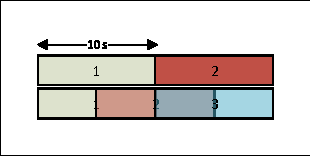
\includegraphics[clip=true, trim=5mm 5mm 5mm 5mm]{img/interval_overlap}
\caption{Intervallüberlappung}
\label{fig:interval-overlap}
\end{figure}

Bao et al. nutzten 2004 auf der Basis bereits bestehender Werke für die Transformation eine Intervallüberlappung von $50 \%$ \cite{Bao2004}. Weiss et al. probierten dies laut ihrem Paper nicht aus \cite{Weiss2016}. Um zu prüfen, ob dies eine weitere Verbesserung der Genauigkeiten erzielen könnte, wurden für die Intervalle $(t_0, t_0 + 10), ((t_0 + 10) - 10 * 0.5, (t_0 + 10) - 10 * 0.5 + 10), ...$ Features generiert und wie zuvor evaluiert. Eine Illustration der Überlappung befindet sich in Abbildung~\ref{fig:interval-overlap}.

Anders als erhofft verschlechterten sich die persönlichen RF-Modelle wie in Tabelle~\ref{tab:accuracy-overlap} ersichtlich durch die Überlappung um $0.2 \%$, während sich die unpersönlichen Modelle sogar um $5.1 \%$ verschlechterten.

\begin{table}
\centering
\begin{tabular}{|c|c|c||c|c|}
	\hline 
	\textbf{Algo.} & \textbf{Comb, Pers.} & \textbf{Überlapp., Pers.} &\textbf{Comb, Unpers.} & \textbf{Überlapp., Unpers.} \\ 
	\hline 
	RF & \textbf{99.4} & \textbf{99.2} & \textbf{78.5} & \textbf{73.4} \\ 
	J48 & 92.8 & 96.3 & 59.7 & 57.5 \\ 
	IB3 & 82.3 & 81.8 & 52.9 & 50.7 \\ 
	NB & 96.2 & 95.8 & 60.9 & 59.7 \\ 
	MLP & 94.8 & 95.0 & 54.9 & 59.4 \\ 
	\hline 
	$\varnothing$ & 93.1 & 93.6 & 61.4 & 60.9 \\ 
	\hline
\end{tabular} 
\caption{Genauigkeit der Modelle mit Intervallüberlappung in Prozent}
\label{tab:accuracy-overlap}
\end{table}

\section{Genauigkeit bei Verschmelzung der Ess- und Trinkaktivitäten}
\begin{table}
\centering
\begin{tabular}{|c|c|c|}
	\hline 
	\textbf{Algo.} & \textbf{Comb, Unpers., verschmolzen} & \textbf{Comb, Unpers., nicht verschmolzen} \\ 
	\hline 
	RF & \textbf{87.1} &  \textbf{78.5} \\ 
	J48 & 73.7 &  59.7 \\ 
	IB3 & 63.9 &  52.9  \\ 
	NB & 72.4 & 60.9  \\ 
	MLP & 77.6  & 54.9 \\ 
	\hline 
	$\varnothing$ & 74.9 & 61.4  \\ 
	\hline
\end{tabular} 
\caption{Genauigkeit der Modelle bei Verschmelzung der Ess- und Trinkaktivitäten in Prozent}
\label{tab:accuracy-merge-eating}
\end{table}
\begin{sidewaystable}
\centering
\begin{tabular}{|c|c|c|c|c|c|c|c|c|c|c|c|c|c|c|c|c|c||l|}
\hline 
\textbf{a} &  \textbf{b} & \textbf{c} & \textbf{d} & \textbf{e} & \textbf{f} & \textbf{g} & \textbf{h} & \textbf{i} & \textbf{j} & \textbf{k} & \textbf{l} & \textbf{m} & \textbf{n} & \textbf{o} & \textbf{p} & \textbf{q} & \textbf{r} & \textbf{$<$ Output für $\vee$} \\
\hline 
\hline 
149 & 0 & 0 & 0 & 0 & 0 & 2 & 0 & 0 & 8 & 0 & 0 & 0 & 2 & 0 & 0 & 0 & 0 & \textbf{a = Brushing Teeth} \\
\hline 
0 & 153 & 0 & 7 & 0 & 0 & 0 & 0 & 0 & 0 & 0 & 0 & 0 & 1 & 0 & 0 & 0 & 0 & \textbf{b = Clapping} \\
\hline 
0 & 0 & 126 & 0 & 0 & 0 & 0 & 0 & 0 & 0 & 0 & 1 &17 & 0 & 0 & 0 & 0 & 26 & \textbf{c = Climbing Stairs} \\
\hline 
0 & 11 & 0 & 147 & 0 & 0 & 0 & 0 & 0 & 1 & 0 & 0 & 0 & 5 & 0 & 0 & 0 & 0 & \textbf{d = Basketball} \\
\hline 
0 & 0 & 0 & 0 & \cellcolor{lightgray} 133 & \cellcolor{lightgray} 6 & \cellcolor{lightgray} 0 & \cellcolor{lightgray} 9 & \cellcolor{lightgray}  0 & 0 & 0 & 0 & 0 & 0 & 12 & 0 & 3 & 0 & \textbf{e = Drinking} \\
\hline 
1 & 0 & 0 & 0 & \cellcolor{lightgray} 5 & \cellcolor{lightgray} 135 & \cellcolor{lightgray} 3 & \cellcolor{lightgray} 15 & \cellcolor{lightgray} 4 & 0 & 0 & 0 & 0 & 0 & 0 & 0 & 1 & 0 & \textbf{f = Eating Chips} \\
\hline 
3 & 0 & 0 & 0 & \cellcolor{lightgray} 0 & \cellcolor{lightgray} \cellcolor{lightgray} 11 & \cellcolor{lightgray} 106 & \cellcolor{lightgray} 3 & \cellcolor{lightgray} 24 & 0 & 3 & 0 & 0 & 0 & 2 & 0 & 9 & 0 & \textbf{g = Eating Pasta} \\
\hline 
3 & 0 & 0 & 0 & \cellcolor{lightgray} 14 & \cellcolor{lightgray} 26 & \cellcolor{lightgray} 15 & \cellcolor{lightgray} 75 & \cellcolor{lightgray} 27 & 0 & 6 & 0 & 0 & 0 & 7 & 1 & 3 & 0 & \textbf{h = Eating Sandwich} \\
\hline 
7 & 0 & 0 & 0 & \cellcolor{lightgray} 0 & \cellcolor{lightgray} 13 & \cellcolor{lightgray} 39 & \cellcolor{lightgray} 44 & \cellcolor{lightgray} 84 & 0 & 0 & 0 & 0 & 0 & 3 & 0 & 2 & 0 & \textbf{i = Eating Soup} \\
\hline 
6 & 0 & 0 & 0 & 0 & 0 & 0 & 0 & 0 & 148 & 0 & 0 & 3 & 2 & 0 & 0 & 0 & 0 & \textbf{j = Folding Clothes} \\
\hline 
0 & 0 & 0 & 0 & 0 & 5 & 7 & 6 & 2 & 0 & 139 & 0 & 0 & 0 & 0 & 0 & 4 & 0 & \textbf{k = Handwriting} \\
\hline 
0 & 0 & 2 & 0 & 0 & 0 & 0 & 0 & 0 & 0 & 0 & 166 & 0 & 0 & 0 & 0 & 0 & 0 & \textbf{l = Jogging} \\
\hline 
0 & 0 &13 & 0 & 0 & 0 & 0 & 0 & 0 & 0 & 0 & 1 & 150 & 0 & 0 & 0 & 0 & 2 & \textbf{m = Soccer Ball} \\
\hline 
0 & 0 & 0 & 7 & 0 & 0 & 0 & 0 & 0 & 0 & 0 & 0 & 3 & 145 & 0 & 0 & 0 & 0 & \textbf{n = Playing Catch} \\
\hline 
4 & 0 & 0 & 0 & 1 & 2 & 2 & 1 & 1 & 0 & 4 & 0 & 0 & 0 & 136 & 8 & 5 & 0 & \textbf{o = Sitting} \\
\hline 
1 & 0 & 0 & 0 & 0 & 0 & 0 & 1 & 0 & 0 & 0 & 0 & 1 & 0 &15 & 142 & 0 & 0 & \textbf{p = Standing} \\
\hline 
2 & 0 & 0 & 0 & 1 & 1 & 4 & 1 & 0 & 0 & 27 & 0 & 0 & 0 & 0 & 0 & 125 & 0 & \textbf{q = Typing} \\
\hline 
0 & 0 &66 & 0 & 0 & 0 & 0 & 0 & 0 & 0 & 0 & 0 & 19 & 0 & 0 & 0 & 0 & 84 & \textbf{r = Walking} \\
\hline 
\end{tabular}
\caption{Konfusionsmatrix der unpersönlichen RF-Modelle}
\label{tab:confusion-impersonal-rf}
\end{sidewaystable}

Betrachtet man die Konfusionsmatrix der vollständigen unpersönlichen RF-basierten Modelle in Tabelle~\ref{tab:confusion-impersonal-rf}, so lässt sich feststellen, dass die Klassen, die sich mit Essen oder Trinken beschäftigen, nur ungenau erkannt werden und somit die Durchschnittsgenauigkeit entsprechend senken. Zudem liegt die fehlerhaft vorhergesagte Klasse in $298/324 \approx 92 \%$ der Fälle im Bereich des Essens und Trinkens. Zurückzuführen ist dies auf die Tatsache, dass sich diese Aktivitäten untereinander ähneln, da die zentralen Bewegungsmerkmale bei all diesen Klassen das Sitzen sowie das Führen der Hand zum Mund sind.

\begin{sidewaystable}
\centering
\begin{tabular}{|c|c|c|c|c|c|c|c|c|c|c|c|c|c||l|}
	\hline 
  \textbf{a} &   \textbf{b} &   \textbf{c} &   \textbf{d} &   \textbf{e} &   \textbf{f} &   \textbf{g} &   \textbf{h} &   \textbf{i} &   \textbf{j} &   \textbf{k} &   \textbf{l} &   \textbf{m}  &  \textbf{n} & \textbf{$<$ Output für $\vee$} \\
\hline 
\hline
143 &   0 &   0 &   0 &   5 &  12 &   0 &   0 &   0 &   1 &   0 &   0 &   0  &  0 &   \textbf{a = Brushing Teeth} \\
\hline 
0 & 155 &   0 &   5 &   0 &   0 &   0 &   0 &   0 &   1 &   0 &   0 &   0  &  0 &   \textbf{b = Clapping} \\
\hline 
0 &   0 & 126 &   0 &   0 &   0 &   0 &   1 &  13 &   0 &   0 &   0 &   0  & 30 &   \textbf{c = Climbing Stairs} \\
\hline 
0 &   5 &   0 & 136 &   0 &   5 &   0 &   0 &   0 &  18 &   0 &   0 &   0  &  0 &   \textbf{d = Basketball} \\
\hline 
2 &   0 &   0 &   0 & 830 &   0 &   2 &   0 &   0 &   0 &  16 &   0 &   7  &  0 &   \textbf{e = Eating} \\
\hline 
2 &   0 &   0 &   0 &   0 & 155 &   0 &   0 &   0 &   2 &   0 &   0 &   0  &  0 &   \textbf{f = Folding Clothes} \\
\hline 
0 &   0 &   0 &   0 &  30 &   0 & 124 &   0 &   0 &   0 &   0 &   0 &   9  &  0 &   \textbf{g = Handwriting} \\
\hline 
0 &   0 &   0 &   0 &   0 &   0 &   0 & 168 &   0 &   0 &   0 &   0 &   0  &  0 &   \textbf{h = Jogging} \\
\hline 
0 &   0 &   6 &   0 &   0 &   0 &   0 &   1 & 157 &   1 &   0 &   0 &   0  &  1 &   \textbf{i = Soccer Ball} \\
\hline 
0 &   0 &   0 &   7 &   0 &   2 &   0 &   1 &   2 & 143 &   0 &   0 &   0  &  0 &   \textbf{j = Playing Catch} \\
\hline 
1 &   0 &   0 &   0 &  23 &   0 &   2 &   0 &   0 &   0 & 130 &   8 &   0  &  0 &   \textbf{k = Sitting} \\
\hline 
0 &   0 &   0 &   0 &   5 &   0 &   0 &   0 &   0 &   0 &  17 & 138 &   0  &  0 &   \textbf{l = Standing} \\
\hline 
1 &   0 &   0 &   0 &  37 &   0 &  18 &   0 &   0 &   0 &   0 &   0 & 105  &  0 &   \textbf{m = Typing} \\
\hline 
0 &   0 &  60 &   0 &   0 &   0 &   0 &   0 &  26 &   0 &   0 &   0 &   0  & 83 &   \textbf{n = Walking} \\
	\hline 
\end{tabular}
\caption{Konfusionsmatrix der unpersönlichen, verschmolzenen RF-Modelle}
\label{tab:confusion-impersonal-rf-merged}
\end{sidewaystable}

Tabelle~\ref{tab:accuracy-merge-eating} zeigt, wie sich die Genauigkeit der unpersönlichen Modelle verändert, wenn man diese Aktivitäten zu einer einzigen Aktivität verschmilzt. Bei den RF-Modellen ist eine Verbesserung um $8.6 \%$ zu erkennen, wovon ein Teil auch darauf zurückzuführen sein könnte, dass es insgesamt weniger Klassen gibt und die Wahrscheinlichkeit einer Fehlklassifikation somit sinkt. Tabelle~\ref{tab:confusion-impersonal-rf-merged} zeigt die neue Konfusionsmatrix der RF-Modelle und es wird deutlich, dass aufgrund der verschmolzenen Aktivität \textit{Eating} die Fehlerrate stark gesunken ist.

Aus diesen Daten lässt sich schließen, dass bei der Verwendung von unpersönlichen Modellen darauf geachtet werden sollte, dass die zu erkennenden Aktivitäten nicht zu feingranular voneinander getrennt werden, da dies die Klassifikation stark erschweren kann.

\section{Genauigkeit in Abhängigkeit von der Teilnehmeranzahl}
\begin{figure}
\centering
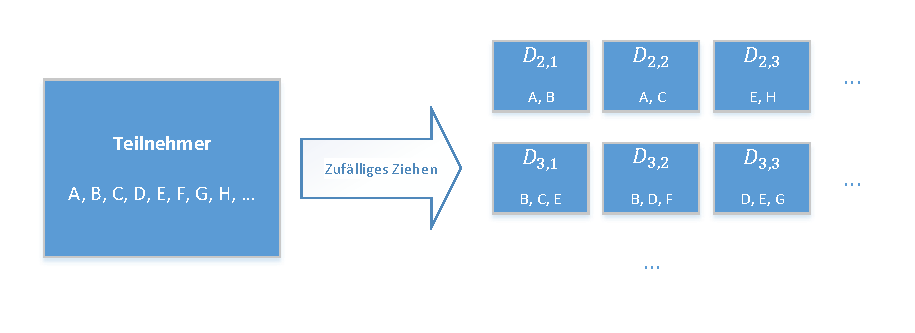
\includegraphics[clip, trim=7mm 7mm 7mm 6mm, width=\textwidth]{img/random-set-draw}
\caption{Ziehung der Datensätze $D_{i,j}$}
\label{fig:random-set-draw}
\end{figure}

Während die persönlichen Modelle lediglich auf die Bewegungsdaten einer einzelnen Person zurückgreifen, sind für die unpersönlichen Modelle Daten anderer Personen erforderlich. Daraus ergibt sich die Frage, wie die Genauigkeit der unpersönlichen Modelle von der Anzahl der Personen, auf denen dieses basiert, abhängig ist. Um dies zu ermitteln, wurden aus dem aus 10 Personen bestehenden vollständigen Datensatz $D$ für $i \in \{2, ..., 10\}$ je $N_i := \min(10, \binom{10}{i})$ verschiedene, zufällig gezogene Datensätze $D_{i,j}$ mit $j \in \{1, ..., N_i\}$ generiert. Dieser Prozess ist in Abbildung~\ref{fig:random-set-draw} illustriert. Ein Datensatz $D_{i,j}$ enthält Daten von $i \geq 2$ verschiedenen Personen, um die Aufteilung in Train- und Testsets zu ermöglichen, da ein Testset für die unpersönlichen Modelle genau eine Person enthalten soll und die Mengen disjunkt sein müssen (vgl. Abschnitt~\ref{subsec:eval-impersonal-models}). Die Genauigkeit in Abhängigkeit von der Anzahl der Personen $i$ ist dann definiert durch $G(i) := \sum_{j=1}^{N_i} \frac{\text{Genauigkeit mit } D_{i,j}}{N_i}$. Die Berechnung der Genauigkeit mit Datensatz $D_{i,j}$ erfolgt nach Abschnitt~\ref{subsec:eval-impersonal-models}.
Abbildung~\ref{fig:accuracy-convergence} zeigt den Plot der Funktion $G$. Es ist zu erkennen, dass die Genauigkeit langsam konvergiert, wobei für $i > 10$ noch etwas höhere Genauigkeiten zu erwarten sind. Die Verifikation dieser Hypothese durch weitere Aufnahmen war im Rahmen der zeitlichen Beschränkungen einer Bachelorarbeit nicht möglich.

Zum Vergleich befindet sich in Abbildung~\ref{fig:accuracy-convergence-lockhart} eine Grafik aus \cite{Lockhart2014}, die zeigt, wie sich die Genauigkeit unpersönlicher RF-Modelle, die nur aus Daten eines Smartphone-Accelerometers gewonnen wurden, in dieser Arbeit in Abhängigkeit von der Personenanzahl verhält. Der große HASC-Datensatz konvergiert gegen eine Genauigkeit von etwa $85 \%$, die laut Extrapolation der Autoren auch mit einem größeren eigenen Datensatz hätten erreicht werden können. Es fällt auf, dass auch der Plot in Abbildung~\ref{fig:accuracy-convergence} gegen einen ähnlichen Grenzwert konvergieren könnte, wobei zu beachten ist, dass die beiden externen Datensätze weniger verschiedene Aktivitäten beinhalten, die zudem hinsichtlich ihrer Erkennbarkeit durch ML-Klassifikation variieren könnten. Zusätzlich ist festzustellen, dass die Genauigkeit in Abbildung~\ref{fig:accuracy-convergence} bei 10 Personen bereits etwa $80 \%$ beträgt, während es in Abbildung~\ref{fig:accuracy-convergence-lockhart} nur etwa $63 \%$, respektive $70 \%$ sind. Dies deutet darauf hin, dass mehr Sensoren die Notwendigkeit vieler Personen im Datensatz verringern.

\begin{figure}
\centering
\begin{tikzpicture}
\begin{axis}[
grid=major, % Display a grid
grid style={dashed,gray!30}, % 
ymin=0,
ymax=100,
xmin=1,
xlabel=$i \text{ = Anzahl der Personen}$,
ylabel=$G(i) \text{ = Genauigkeit der Modelle}$]
\addplot[color=black,mark=x] coordinates {
	(2, 52.52308602)
	(3, 64.3778887)
	(4, 67.2191227465409)
	(5, 72.94877937)
	(6, 73.61805308)
	(7, 74.9440529)
	(8, 76.93207282)
	(9, 76.83383234)
	(10, 79.919409)
};
\end{axis}
\end{tikzpicture}
\caption{Genauigkeit in Abhängigkeit von der Personenanzahl}
\label{fig:accuracy-convergence}
\end{figure}
\todo{Check if this figure is in the right place}

\begin{figure}
\centering
\includegraphics[clip, trim=22mm 197mm 22mm 27mm, page=8, width=\textwidth]{img/Lockhart2014}
\caption{Genauigkeit in Abhängigkeit von der Personenzahl (Lockhart \& Weiss \cite{Lockhart2014})}
\label{fig:accuracy-convergence-lockhart}
\end{figure}

\section{Optimierung der Hyperparameter}
Um die unpersönlichen Modelle weiter zu verbessern, wurden die Hyperparameter des RF-Modells optimiert, da dieses Verfahren bis dato das beste Ergebnis geliefert hat. Als Baseline dient das RF1-Modell, das dieselben Hyperparameter besitzt wie das RF-Modell in Abbildung~\ref{tab:accuracy-impersonal}. Zu bemerken ist, dass die folgenden Genauigkeiten je nach Seed für den Zufallsgenerator um $\pm 1.5 \%$ schwanken, weshalb die Genauigkeit des RF1-Modells im hier gezeigten Durchlauf des Tests rund $1.45 \%$ über der des RF-Modells in Abbildung~\ref{tab:accuracy-impersonal} liegt.

Die variierten Hyperparameter sind die folgenden:

\begin{itemize}
	\item \textit{numIterations} gibt die Anzahl der Entscheidungsbäume im Wald an. Ein zu niedriger Wert sorgt dafür, dass die zufällig generierten Bäume den Datensatz zusammen nicht gut genug abdecken können.
	\item \textit{numFeatures} gibt die Anzahl der Features an, die jeder Entscheidungsbaum bei einem Split betrachtet. Wird ein zu hoher Wert verwendet, ist die Entwicklung des Baums weniger vom Zufall getrieben. Ist der Wert zu niedrig, so sinkt die Wahrscheinlichkeit, dass ein Split an einem Feature durchgeführt wird, sodass der Information Gain groß ist.
	\item \textit{maxDepth} bestimmt die maximale Tiefe der Entscheidungsbäume im Wald. Ein niedriger Wert sorgt dafür, dass der Baum sich den Trainingsdaten nicht zu sehr anpasst und overfittet. Dabei muss beachtet werden, dass ein zu niedriger Wert wiederum dafür sorgen kann, dass zu wenige Features betrachtet werden können, um eine genaue Klassifizierung zu ermöglichen.
\end{itemize}

Tabelle~\ref{tab:hyperparam-opt} zeigt die Genauigkeiten in Abhängigkeit von den Hyperparametern. In einigen Fällen wurde für \textit{numFeatures} der WEKA-Standardwert $f = \lfloor log_2(n - 1) + 1 \rfloor = \lfloor log_2(208) + 1 \rfloor = 8$ verwendet wird, wobei $n$ die Anzahl der Features einer Instanz ist.

Gegenüber der Baseline ist das RF8-Modell das beste, allerdings nur weniger als $1.3 \%$ besser, sodass die Differenz unter den Veränderungen durch Schwankungen liegt. Es ist jedoch festzustellen, dass der automatisch gewählte Wert $f$ für \textit{numFeatures} die besten Ergebnisse erzielt. Eine Erhöhung der maximalen Tiefe auf 50 oder gar 75 erzielt keine nennenswert besseren Ergebnisse als die oben gewählte Tiefe von 25. Auch für die Anzahl der Bäume gilt, dass bereits 50 annähernd so gut sind wie 100 oder mehr. Positiv zu vermerken ist somit, dass in diesem Anwendungsfall von Random Forests auch kleine Werte eine gute Genauigkeit liefern, wobei der Leistungsbedarf entsprechend niedriger ist.

\begin{table}
\centering
\begin{tabular}{|c|c|c|c||c|}
	\hline 
	& \textbf{numIterations} & \textbf{numFeatures} & \textbf{maxDepth} & \textbf{Genauigkeit} \\ 
	\hline 
	\textbf{RF8} & 75 & $f$ & 50 & 81.229 \\ 
	\hline 
	\textbf{RF7} & 100 & $f$ & 75 & 80.7925 \\ 
	\hline 
	\textbf{RF4} & 100 & $f$ & 50 & 80.6917 \\ 
	\hline 
	\textbf{RF6} & 150 & $f$ & 50 & 80.1545 \\ 
	\hline 
	\textbf{RF9} & 100 & $f$ & 30 & 80.0537 \\ 
	\hline 
	\textbf{RF1} & 50 & 10 & 25 & 79.953 \\ 
	\hline 
	\textbf{RF2} & 200 & $\infty$ & $\infty$ & 73.5729 \\ 
	\hline 
	\textbf{RF5} & 200 & $\infty$ & 50 & 73.2371 \\ 
	\hline 
	\textbf{RF3} & 200 & $\infty$ & 50 & 72.6998 \\ 
	\hline
\end{tabular}
\caption{Hyperparameteroptimierung}
\label{tab:hyperparam-opt}
\end{table}

\section{Einfluss von Feature-Selection}
Betrachtet man die \textit{Comb}-Spalte in Tabelle~\ref{tab:accuracy-impersonal}, so fällt auf, dass die Genauigkeiten der übrigen Modelle dem RF-Modell deutlich unterlegen sind. Da dies bei den persönlichen Modellen nicht der Fall ist, und es somit kein inhärentes Problem mit der Art der Daten zu geben scheint, ist es untersuchenswert, ob die anderen Algorithmen nicht durch eine Vorauswahl der Features (\textit{Feature Selection}) höhere Genauigkeiten liefern können, da eine solche Auswahl prinzipiell auch durch den Zufall im Random Forest erfolgt.

Zur Feature Selection wurde das Verfahren \textit{CfsSubsetEval}\cite{Hall1998} verwendet, das laut WEKA-Dokumentation wie folgt arbeitet:

\begin{quote}
	"[CfsSubsetEval] ermittelt den Wert einer Untermenge der Features, indem die individuelle Vorhersagefähigkeit eines jeden Features mitsamt dem Grad der Redundanz zwischen ihnen betrachtet wird. Feature-Untermengen, die stark mit der Klasse korrelieren und dabei eine niedrige Interkorrelation haben, werden bevorzugt."
	
	\textit{-- aus \cite{WekaCfsSubsetEval} übersetzt.}
\end{quote}

Begonnen wurde mit der leeren Menge, der nach und nach Features hinzugefügt worden sind, bis die Bewertung durch \textit{CfsSubsetEval} sank.

Unter Einsatz der Feature Selection entstanden die Ergebnisse aus Tabelle~\ref{tab:accuracy-feature-selection}. Gegenüber Tabelle~\ref{tab:accuracy-impersonal} sind die Genauigkeiten der IB3-, NB- und MLP-Modelle wesentlich besser, wodurch auch der Durchschnittswert angehoben wird, jedoch schlägt weiterhin kein Algorithmus den RF-Algorithmus. Diesen hat die Feature Selection des Weiteren nicht verbessert, sodass sich die Feature Selection in diesem Anwendungsszenario als nicht sinnvoll erwiesen hat.

\begin{table}
\centering
\begin{tabular}{|c|c|}
	\hline 
	\textbf{Algo.} & \textbf{Comb, Unpers.} \\ 
	\hline 
	RF & 78.2 \\ 
	J48 & 60.0 \\ 
	IB3 & 59.6 \\ 
	NB & 67.8 \\ 
	MLP & 68.3 \\ 
	\hline 
	$\varnothing$ & 66.8 \\ 
	\hline 
\end{tabular}
\caption{Genauigkeit mit Feature Selection}
\label{tab:accuracy-feature-selection}
\end{table}

\section{Wahl der Intervallgröße}
Dernbach et al. zeigten 2012, dass die Wahl der Intervallgröße einen Einfluss von circa $5 \%$ auf die Genauigkeit der Erkennung komplexer Aktivitäten haben kann \cite{Dernbach2012}, wodurch die Anstrengung motiviert wurde, auch in dieser Arbeit verschiedene Möglichkeiten der Intervallwahl zu überprüfen. \todo{TODO}

% vim: set ft=tex

\chapter{Fazit}
\label{chap:conclusions}
\todo{Check template for suggestions on how to write all of this}

\section{Zusammenfassung}
\todo{TODO}

\section{Beurteilung der Ergebnisse}
\todo{TODO}

\section{Zusammenhang zum Kontext}
\todo{TODO}

\section{Ausblick}
\todo{TODO}

\section{Reflexion}
\todo{TODO}


% vim: set ft=tex


\appendix
\part*{\appendixname}
% \chapter{What goes in the appendices}


% vim: set ft=tex

\chapter{Verwendete Akronyme}
\label{chap:acronyms}
\begin{acronym}[AAAA]
    \acro{ML}{Machine Learning}
    \acro{RF}{Random Forest}
    \acro{IB}{Instance-Based-Learner / IB\textit{k}}
    \acro{J48}{J48-Entscheidungsbaum}
    \acro{NB}{Naive Bayes}
    \acro{MLP}{Multilayer Perceptron}
    \acro{NTP}{Network Time Protocol}
    \acro{SDK}{Software Development Kit}
    \acro{HASC}{Human Activity Sensor Consortium}
    \acro{JSON}{JavaScript Object Notation}
    \acro{GZIP}{GNU zip}
\end{acronym}

% vim: set ft=latex


% Bibliography
\bibliographystyle{plain}
\bibliography{thesis}
%
\backmatter
\input{erklaerung}
%
\end{document}
%EOF
% vim: set ft=tex
